% !TeX program = xelatex
\documentclass[UTF8,fontset=fandol,10pt,a4paper]{ctexart}
\usepackage[left=22mm,right=22mm,top=23mm,bottom=22mm,headheight=14pt]{geometry}
\usepackage{fontspec}
\setmainfont{TeX Gyre Heros}
\setsansfont{TeX Gyre Heros}
\setmonofont{Latin Modern Mono}
\renewcommand{\familydefault}{\sfdefault}
\usepackage[table]{xcolor}
\usepackage{graphicx,tikz}
\usetikzlibrary{arrows.meta,positioning,fit,backgrounds,calc}
\usepackage{booktabs,tabularx,array,enumitem,float,caption,fancyhdr,hyperref}
\definecolor{blue}{HTML}{2869A9}
\definecolor{ink}{HTML}{293340}
\definecolor{muted}{HTML}{647181}
\definecolor{line}{HTML}{C5D4E2}
\definecolor{pale}{HTML}{F0F5FA}
\definecolor{warm}{HTML}{FFF7E9}
\hypersetup{colorlinks=true,urlcolor=blue,linkcolor=blue,pdftitle={Redflag RHI 与 Vulkan 接入设计},pdfauthor={Redflag}}
\color{ink}
\setlength{\parindent}{0pt}
\setlength{\parskip}{6pt}
\linespread{1.16}
\setlist[itemize]{leftmargin=1.5em,itemsep=2pt,topsep=3pt}
\setlist[enumerate]{leftmargin=1.8em,itemsep=3pt,topsep=3pt}
\renewcommand{\arraystretch}{1.38}
\newcolumntype{Y}{>{\raggedright\arraybackslash}X}
\newcolumntype{L}[1]{>{\raggedright\arraybackslash}p{#1}}
\ctexset{section={format=\Large\bfseries\color{blue},beforeskip=16pt,afterskip=8pt},subsection={format=\large\bfseries\color{blue},beforeskip=11pt,afterskip=5pt}}
\captionsetup{font=small,labelfont=bf,textfont={color=muted},skip=7pt}
\pagestyle{fancy}\fancyhf{}
\fancyhead[L]{\small\color{muted}Redflag · RHI / Vulkan · 设计方案}
\fancyhead[R]{\small\color{muted}2026-11-21}
\fancyfoot[C]{\small\color{muted}\thepage}
\renewcommand{\headrulewidth}{0pt}
\newcommand{\note}[1]{{\small\color{muted}#1\par}}
\newcommand{\code}[1]{{\small\texttt{#1}}}
\newcommand{\ruleline}{\par\vspace{4pt}{\color{line}\hrule}\vspace{8pt}}
\newcommand{\source}[2]{{\small\href{#1}{[#2]}}}
\tikzset{
 module/.style={draw=line,fill=pale,rounded corners=2pt,align=center,inner sep=7pt,text width=3.8cm,minimum height=1.15cm,font=\small},
 smallbox/.style={module,text width=2.55cm,minimum height=.95cm,font=\footnotesize},
 wide/.style={module,text width=9.5cm},
 planned/.style={module,fill=warm,dashed},
 flow/.style={-{Stealth[length=2mm]},draw=muted,line width=.65pt},
 own/.style={flow,dashed},
 label/.style={font=\scriptsize,fill=white,inner sep=2pt,text=muted}}

% 本册的页幅、图注和代码排版。
\geometry{paperwidth=190mm,paperheight=252mm,left=21mm,right=21mm,
  top=22mm,bottom=21mm,headheight=21pt,headsep=4mm,footskip=10mm}
\usepackage{amsmath,listings,type1cm}
\definecolor{Ink}{HTML}{202E33}
\definecolor{Muted}{HTML}{4C6064}
\definecolor{Teal}{HTML}{12665F}
\definecolor{Rust}{HTML}{9E452B}
\definecolor{Rule}{HTML}{B3C6C1}
\definecolor{Soft}{HTML}{EAF3F0}
\definecolor{Paper}{HTML}{FFFFFF}
\setmainfont{TeX Gyre Pagella}
\renewcommand{\familydefault}{\rmdefault}
\linespread{1}
\setcounter{secnumdepth}{0}
\setlength{\emergencystretch}{2em}
\setlength{\parindent}{0pt}
\setlength{\parskip}{5.8pt}
\ctexset{section={format=\raggedright\sffamily\bfseries\fontsize{23}{30}\selectfont\color{Ink},
    beforeskip=0pt,afterskip=9pt},
  subsection={format=\raggedright\sffamily\bfseries\fontsize{13}{18}\selectfont\color{Teal},
    beforeskip=8pt,afterskip=2pt}}
\hypersetup{urlcolor=Teal,linkcolor=Teal,bookmarksnumbered=false,
  pdfsubject={Redflag 渲染接口、后端实现与验证}}
\fancyhf{}
\setlength{\headwidth}{\textwidth}
\fancyhead[L]{\sffamily\fontsize{9.5}{12}\selectfont\bfseries\color{Teal}Redflag\enspace{\mdseries\color{Muted}图形引擎}}
\fancyhead[R]{\sffamily\small\color{Muted}RHI / Vulkan}
\renewcommand{\headrule}{\hbox to\headwidth{\color{Rule}\leaders\hrule height .55pt\hfill}}
\fancyfoot[L]{\small\sffamily\color{Muted}\nouppercase{\leftmark}}
\renewcommand{\sectionmark}[1]{\markboth{#1}{}}
\fancyfoot[R]{\large\sffamily\bfseries\color{Teal}\thepage}
\renewcommand{\code}[1]{{\ttfamily\fontsize{10.4}{14}\selectfont #1}}
\newcommand{\readings}[1]{\par\noindent{\sffamily\fontsize{9.6}{14}\selectfont
  \color{Muted}参考\enspace #1\par}}
\newcommand{\refitem}[2]{\href{#1}{#2}}
\newcommand{\figpanel}[2]{\begin{figure}[H]\centering\input{figures/#1}\caption{#2}\end{figure}}
\DeclareCaptionFont{rhicapt}{\sffamily\fontsize{10}{14}\selectfont\color{Muted}}
\captionsetup{font=rhicapt,labelfont={bf,color=Teal},textfont=rhicapt,
  labelsep=quad,justification=raggedright,singlelinecheck=false,skip=4pt}
\setlength{\intextsep}{7pt plus 1pt minus 1pt}
\lstset{basicstyle=\ttfamily\fontsize{10.7}{15}\selectfont\color{Ink},
  backgroundcolor=\color{Soft},frame=l,rulecolor=\color{Teal},framerule=1.5pt,
  xleftmargin=5mm,xrightmargin=2mm,framexleftmargin=3mm,framesep=2pt,
  aboveskip=6pt,belowskip=6pt,columns=fullflexible,keepspaces=true,showstringspaces=false}
\newcommand{\bodytype}{\normalfont\fontsize{11.4}{17.8}\selectfont\color{Ink}}

\input{build/timing-rows}
\hypersetup{pdftitle={Redflag 渲染性能实测},pdfsubject={OpenGL 绘制、Vulkan 光照与屏幕效果}}
\fancyhead[R]{\sffamily\small\color{Muted}OpenGL / 性能实测}
\graphicspath{{../../../output/profiling/}}
\newcommand{\smalltable}{\sffamily\fontsize{10.3}{14}\selectfont\renewcommand{\arraystretch}{1.35}}
\newcommand{\panelimage}[3]{\begin{minipage}[t]{#1}\centering\vspace{0pt}#2\par
  \vspace{2pt}{\small\sffamily\color{Muted}#3\par}\end{minipage}}
\begin{document}
\bodytype
\section{渲染性能实测}
同是画 64 个四边形，2D 渲染器可以把它们的顶点拼在一起，3D 渲染器可以让同一份网格在 64 个位置各画一次。两种做法都能减少绘制调用。深度预写（Pre-Z）恰好在做相反的交换：先多画一遍，换取主绘制少处理一些被挡住的像素。这次在同一台电脑上把三项分别做了对照。

\subsection{一次提交和一次绘制各用了多久}
{\smalltable\begin{tabularx}{\linewidth}{@{}Xrrrr@{}}\toprule
&\multicolumn{2}{c}{CPU 提交（微秒）}&\multicolumn{2}{c}{GPU 区间（微秒）}\\
\cmidrule(lr){2-3}\cmidrule(l){4-5}
同一画面的画法 & 中位数 & P10--P90 & 中位数 & P10--P90\\\midrule
\drawTimingRows
\bottomrule\end{tabularx}\par}
每种画法先预热 30 帧，再记录 120 帧，轮换每轮先执行的画法。中位数表示有一半样本用时比它短。P10 到 P90 是中间八成样本所在的区间。横向读同一行，可以区分 CPU 发出命令和显卡完成这段工作的时间；比较两种画法，则在同一组内纵向读。

二维和三维各自使用固定的 $256\times256$ 离屏目标。设备为 Ryzen 9 8945HX、RTX 5070 Ti Laptop GPU，Windows 平衡电源方案，OpenGL 4.6，NVIDIA 驱动 616.56，Debug/x64。计时时不加载 RenderDoc。CPU 从清屏和组织绘制开始计，最后一次提交返回就停表。GPU 用 \code{GL\_TIME\_ELAPSED} 测相同命令区间，其中可能包含显卡等待后续命令的空闲时间。

每轮在计时结束后等本帧完成，再开始下一帧。引擎编译时启用了性能埋点。即使关闭日志文件，执行这些函数仍会计时、处理字符串，逐个提交会多次支付这些开销。这里可以比较两种画法在当前构建下的成本，编辑器中的帧率还取决于其他效果、界面与呈现。
\readings{\refitem{https://registry.khronos.org/OpenGL/extensions/ARB/ARB_timer_query.txt}{Khronos · OpenGL 计时查询}\quad
原始样本见 \path{output/profiling/} 下两个实验的 \path{timing.csv}。}

\newpage
\section{2D 精灵的批渲染}
画面里有 64 个精灵，交替使用蓝色十字和黄色菱形两张贴图。第一种画法每个精灵单独开始、结束一次场景。第二种只开始一次场景，等 64 个精灵全部加入后一起绘制。精灵的位置、入队顺序、贴图、透明部分与拾取编号相同。

\begin{figure}[H]\centering
\panelimage{.46\linewidth}{
\includegraphics[width=45mm]{batch2d/individual-half.png}}{事件 323 · 已画出前 32 个}
\hfill
\panelimage{.46\linewidth}{
\includegraphics[width=45mm]{batch2d/batch.png}}{事件 658 · 一次画齐 64 个}
\caption{RenderDoc 回放导出的颜色图。逐个提交结束时（事件 643）的颜色和拾取编号，与右图整幅逐字节相同。}\end{figure}

每个精灵由两个三角形组成，使用 6 个索引。逐个提交能看到 64 次 \code{glDrawElements(6)}。合批把 256 个顶点放进同一批，事件 658 一次读 384 个索引。左右仍各画 128 个三角形。图中的两种图案也都保留了各自的编号，点左上蓝十字读到 57，点旁边的黄菱形读到 58。

\begin{figure}[H]\centering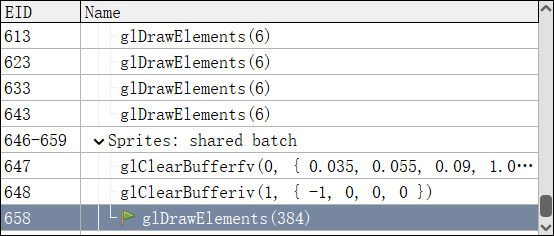
\includegraphics[width=79mm]{batch2d/renderdoc-events.png}
\caption{实际事件列表的末尾。643 结束逐个提交，646 开始合批对照；清空上一幅图后，658 完成整批绘制。}\end{figure}
逐个提交还重复更新相机、上传顶点并绑定资源。第 1 页测得的差额包含这一整套调用。测试只用了两张不同的图，下一步要看一批里出现很多种贴图时，拆批会让开销增加多少。

\newpage
\section{3D 网格的实例化绘制}
同一份几何可以用一组顶点画很多遍。每个实例另存自己的变换和拾取编号，所以第 1 个方块和第 64 个方块可以出现在不同位置。为了让现有引擎走普通绘制路径，对照组创建了 64 份内容相同、对象不同的网格。实例化组的 64 个对象则引用同一份网格。两组在本页都关闭 Pre-Z。

\begin{figure}[H]\centering
{\setlength{\fboxsep}{0pt}\colorbox{Ink}{
\includegraphics[width=49mm]{mesh/final-color.png}}}
\caption{RenderDoc 回放的 3D 颜色输出，透明背景衬以深色。两个模式在全部 65,536 个像素上的 HDR 颜色、实体编号、深度均逐字节相同。}\end{figure}

{\smalltable\begin{tabularx}{\linewidth}{@{}Xrrr@{}}\toprule
主绘制 & 绘制次数 & 每次索引 & 每次实例 \\\midrule
独立网格，事件 24 至 465 & 64 & 6 & 1\\
共享网格，事件 44 & 1 & 6 & 64\\\bottomrule
\end{tabularx}\par}
2D 批渲染把多份顶点拼起来，一次使用 384 个索引。3D 实例化仍然只有 6 个索引，显卡用 64 份实例数据反复画同一张网格。这里两组都留下 43,264 个方块像素，逐点核对编号也能排除“看起来相同，却只能选到一个物体”的错误。

共享网格后 CPU 少提交了 63 条绘制，但还要给物体分组，整理并上传 64 份实例数据。对照组使用不同的网格对象，也会切换对应的顶点数组。因此本次差额包括网格复用、实例化和驱动状态切换的共同影响。场景里有许多不同网格时，要重新测量实际能合成多少组。
{\small\sffamily\color{Muted}原始帧位于 \path{output/profiling/mesh/}。\\
逐个绘制用 \path{separate_capture.rdc}，实例化用 \path{instanced_capture.rdc}。\par}

\newpage
\section{深度预写与遮挡}
在同一排方块上只加一项操作：正式着色前先画深度和法线。预写时关闭场景颜色和实体编号的写入，使用严格的“小于”深度比较。主绘制再允许“等于”通过，同时关闭深度写入。这样同一表面可以着色，并保留刚写好的深度。

\begin{figure}[H]\centering
\panelimage{.32\linewidth}{
\includegraphics[width=39mm]{mesh/prepass-depth.png}}{事件 467 · 预写结束}
\hfill
\panelimage{.63\linewidth}{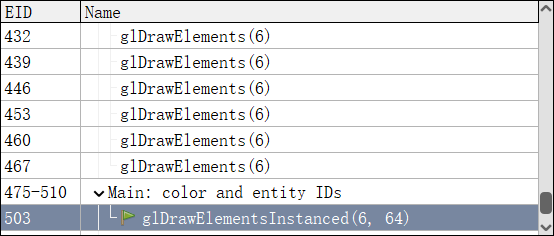
\includegraphics[width=\linewidth]{mesh/renderdoc-events.png}}{事件 503 · 画 64 个实例}
\caption{左图是回放导出的深度，灰色方块为 0.5，白色背景为 1。右图是同一捕获的事件列表，最后一次普通绘制之后紧跟实例化主绘制。}\end{figure}

{\smalltable\begin{tabularx}{\linewidth}{@{}Xrrr@{}}\toprule
回放中的阶段 & 绘制次数 & 三角形 & 片元着色调用 \\\midrule
关闭预写，只画主画面 & 1 & 128 & 43,264\\
开启预写，先写深度和法线 & 64 & 128 & 43,264\\
开启预写，再画主画面 & 1 & 128 & 43,264\\\bottomrule
\end{tabularx}\par}
RenderDoc 的 \code{PS Invocations} 计数记录片元着色器启动了多少次。这些方块彼此分开，预写没有挡住主绘制的任何方块。主绘制的计数完全相同，预写却多执行一遍，整帧的 CPU 和 GPU 区间中位数都变长了。捕获还核实了事件 467 的深度与主绘制结束时逐字节相同。

在完整场景中，近处墙体可能遮住后方的一大片模型，那些像素就有机会省下主着色的成本。SSAO 和 RSM 还要读取深度或法线，现有场景渲染器在它们启用时也会安排预写。单独比较 Pre-Z 的速度时，应先让两组对这些输入的需求相同，再解释差额。
\readings{捕获见 \path{output/profiling/mesh/prepass_capture.rdc}。每个阶段的状态、计数和像素核对见同目录 \path{replay.json}。}

\newpage
\section{下一轮值得测什么}
\subsection{从无遮挡改为前后遮挡}
当前样本里多出的 64 次预写没有省下主着色。下一组保留相同的模型数、材质、投影和分辨率，只改变它们前后重叠的程度，每一种布局分别开关 Pre-Z。记录主绘制省下多少片元着色、预写自己花掉多少 GPU 时间。若主绘制变便宜而整帧仍变慢，再试让共享网格的深度预写也用实例化，同时核对 Mask 材质的透明轮廓和深度。

\subsection{很多小批次的开销}
这次 3D 的 64 个物体恰好能合成一组。可以让物体总数不变，依次改成每个网格只有 1、2、4、8 个实例，比较分组、上传和主绘制的时间，看看两件物体就合批的取舍是否合适。2D 测试则让屏幕布局保持不变，只增加独立贴图数，跨过当前批次的贴图容量。结合事件列表里的拆批位置、CPU 提交时间，以及透明边缘的颜色和编号，判断是否值得调整贴图的组织方式。

\subsection{把候选改法放回编辑器}
这次循环只测离屏绘制。下一次用 Release 构建，编译时关闭性能埋点，再固定 Sponza 的镜头检查遮挡与多材质，固定 Cornell Box 的镜头检查间接光。编辑器的深度预览还会把原尺寸深度图读回 CPU，再生成缩略图。对同一镜头单独开关预览，测 CPU 等待和 GPU 区间。如果读回确实占主要时间，再试直接用着色器显示深度。以上是待验证的方向。

\subsection{复查与复现}
原始帧及回放说明在 \path{output/profiling/batch2d/} 和 \path{output/profiling/mesh/}。用 RenderDoc 打开捕获，另外运行以下脚本计时。
\begin{lstlisting}
REM 在仓库根目录运行。分别保存 2D 合批与 3D 绘制的逐帧计时。
tests\run_sprite_batch.cmd --measure
tests\run_profile_tests.cmd --measure output\profiling\mesh\timing.csv
\end{lstlisting}
编译本册会核对四份原始帧的摘要，再从两份逐帧 CSV 重算首页的表。旧版 Chrome 时间线保存在 \path{output/profiling/}，当时每轮还包含等待和日志写入。
\input{build/compute-timing}
\clearpage
\fancyhead[R]{\sffamily\small\color{Muted}Vulkan / 光照实测}
\ctexset{section={afterindent=true},subsection={afterindent=true}}
\setlength{\parindent}{2\ccwd}
\section{Sponza 中庭的直接光与反射光}
看中庭地面上的一块石板。灯直接照到它，是直接光；灯先照亮柱子，柱子再把光反射到石板上，才算一次间接光。程序把这两部分分开保存。直接光有亮度较高的局部光斑，反射光弱得多，能照到灯光够不到的地方。

\begin{figure}[H]\centering
\panelimage{.48\linewidth}{
\includegraphics[width=\linewidth]{gi/direct-reference.png}}{16 盏灯逐一求和}
\hfill
\panelimage{.48\linewidth}{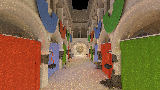
\includegraphics[width=\linewidth]{gi/indirect-reference.png}}{只保留一次反射}
\caption{同一机位、同一套线性材质。为看清较弱的反射，右图显示曝光为 20，左图为 4。下文的误差均从调曝光前的浮点值计算。}
\end{figure}

场景来自 Khronos 示例资产库。测试把 Sponza 的最长边缩放到 20 个场景单位，在通道两侧放置 16 盏暖色和冷色点光。相机位于 $(-5.5,-2.2,0)$，朝向 $(6,-1.8,0)$，垂直视角 $65^\circ$。GPU 用包围盒树查找射线先碰到哪块三角形。为了只比较光照估计，基准里的每个材质用底色贴图的平均线性反射率，忽略透明裁剪，两个方向都能击中三角形。

直接光的对照逐一检查每盏灯能否照到石板，然后把可见灯的贡献加起来。间接光需要知道周围每个方向反射回来多少光。对照为每个可见像素发出两组各 512 条半球射线。每条射线击中另一块表面后，采样一盏灯并检查中间有无遮挡；把两组独立结果平均，得到每像素 1,024 个样本的参考图。两组结果的差异给出约 $1.08\times10^{-5}$ 的参考均方误差估计，参考图本身仍有噪声。

误差在 $160\times90$ 图中的 14,256 个可见像素上计算。对每个像素和三个颜色通道，把测量值减去对应参考值，平方后取平均。这个数越小，说明颜色越接近同一张参考图。实验使用四个随机种子，各种方法共用同一组种子。灯、镜头和几何保持静止。

\readings{\refitem{https://github.com/KhronosGroup/glTF-Sample-Assets/tree/e124e8d8d7330a5372bc2b4d00d39a4a9d7997ea/Models/Sponza}{Khronos · Sponza 模型来源与作者}。\texttt{tests/fetch\_sponza.py} 下载同一版本。}

\clearpage
\section{样本怎样影响亮度与误差}
直接光最简单的近似是每次选一盏灯。若恰好选了柱子后面的灯，这个像素本帧就得零。ReSTIR DI 会把自己的新候选与上一帧、相邻像素的候选一起比较。保留下来的记录叫作样本库（reservoir），里面只存一个选中的候选、累计权重和候选数。来自邻居的灯仍需从当前表面重新检查阴影。下面的 DI 和 GI 每帧每个可见像素各产生一个新候选，另检查最多四个邻居，表中读取运行八帧后的输出。

间接光可以从两条路近似。DDGI 在房间里布置 $12\times6\times7$ 个探针，每个探针向六个朝向分别取 16 条射线，记录反射光和到障碍物的距离。石板从附近八个探针插值，再乘上自身反射率。ReSTIR GI 保存的是光从其他表面反射过来的那段路径。邻像素用到这条路径时，需要重新检查石板能否看见第二块表面，再按新连线的距离与两端角度计算贡献。因此，同一盏灯被柱子挡住与同一段反射路径被柱子挡住，涉及两种不同的可见性检查。

{\noindent\smalltable\begin{tabularx}{\linewidth}{@{}Xrrr@{}}\toprule
估计方法 & 均方误差 & 平均线性 RGB & 复用占比\\\midrule
直接光，每像素 1 个样本 & 0.16609 & 0.10873 & ---\\
直接光，每像素 8 个样本 & 0.02152 & 0.11019 & ---\\
ReSTIR DI，第 8 帧 & 0.01132 & 0.11226 & 91.0\%\\\midrule
反射光，每像素 1 个样本 & 0.02238 & 0.01148 & ---\\
反射光，每像素 8 个样本 & 0.001810 & 0.01115 & ---\\
DDGI，第 8 帧 & 0.0000410 & 0.00904 & ---\\
ReSTIR GI，第 8 帧 & 0.0003678 & 0.01017 & 91.6\%\\\bottomrule
\end{tabularx}\par}

复用占比统计全部可见像素中，最终选中已有候选且确实有光的比例。直接光参考平均为 0.11140，反射光为 0.01110。探针得到的反射光最平滑，平均亮度也比参考低约 18.5\%；ReSTIR GI 低约 8.4\%。表中的每种方法承担的工作不同。探针试验每帧会更新全部探针，样本复用也要付出重新检查遮挡的成本。仅凭误差无法比较每毫秒画出的效果。

\readings{论文与实现范围可对照 \refitem{https://research.nvidia.com/publication/2019-05_dynamic-diffuse-global-illumination-ray-traced-irradiance-fields}{Majercik 等 · DDGI}、
\refitem{https://research.nvidia.com/labs/rtr/publication/bitterli2020spatiotemporal/}{Bitterli 等 · ReSTIR DI} 与
\refitem{https://research.nvidia.com/publication/2021-06_restir-gi-path-resampling-real-time-path-tracing}{Ouyang 等 · ReSTIR GI}。本次实现只测单次漫反射，探针使用六个朝向，样本复用使用有限历史和兼容表面筛选。}

\clearpage
\section{在 RenderDoc 里找回这三种光照}
打开 \path{SponzaGI_capture.rdc}，先选事件 8，再选事件 20。前者把新采到的反射光写入探针，后者按每个可见表面的位置读取相邻探针。接着看事件 44 和 68。它们写同一份像素缓冲区，里面在这两个时刻分别存着直接光和一次反射光。回放脚本分别停在这三个输出时刻，读出每像素四个浮点数，用前三个数生成了下图。

\begin{figure}[H]\centering
\panelimage{.318\linewidth}{
\includegraphics[width=\linewidth]{gi/capture-ddgi.png}}{20 · 探针反射光}
\hfill\panelimage{.318\linewidth}{
\includegraphics[width=\linewidth]{gi/capture-di.png}}{44 · 直接光}
\hfill\panelimage{.318\linewidth}{
\includegraphics[width=\linewidth]{gi/capture-gi.png}}{68 · 路径反射光}
\caption{RenderDoc 1.47 的首帧回放。第三幅还有明显颗粒。本次捕获从空历史开始；上一页比较的两种 ReSTIR 结果已经运行八帧。}
\end{figure}

{\noindent\smalltable\begin{tabularx}{\linewidth}{@{}Xrrrr@{}}\toprule
GPU 执行内容 & 事件 & 工作组数 & 中位数（ms） & 范围（ms）\\\midrule
\giTimingRows\bottomrule\end{tabularx}\par}

在 RTX 5070 Ti Laptop GPU 上先回放一次预热，再读取九轮 RenderDoc 的 GPU 事件计时。每组有 64 个线程，225 组覆盖一整张图。计时只覆盖表中相应的一条计算命令。工程启用 Debug/x64，独立基准的 CPU 计时还包含命令记录、提交和等待，原始数据单列于 \path{trials.csv}。这两种时间都不能直接换算成编辑器帧率。

探针更新明显比在表面查询探针耗时。下一轮可以每次只更新部分探针，把节省的毫秒与移动光源后的追光延迟放在一起比较。另一项可复现实验是固定总 GPU 毫秒，改变反射路径的邻居数，观察柱脚附近的噪声与平均亮度是否改善。这样才能检验增加复用是否值得。

\readings{原始帧、独立结果和逐事件回放记录保存在 \path{output/profiling/gi/}。运行 \path{tests/run_gi_benchmark.cmd} 与 \path{tests/analyze_gi.py} 可重算误差。探针与路径的实现见 \path{GI/Shaders/GI.comp}。}

\clearpage
\section{镜头停下后，哪些像素还在变}
编辑器里曾出现这样的现象：相机已经停下，远处的线条还在晃。为分开检查成因，这组实验改用编辑器场景里的三盏点光和模型纹理，固定 Sponza 的变换与镜头，按旧版预览的 $320\times180$ 连续生成 24 帧。这里可以分别关闭光照采样和相机的亚像素偏移，再看某个像素下一帧究竟变了多少。

\begin{figure}[H]\centering
\panelimage{.318\linewidth}{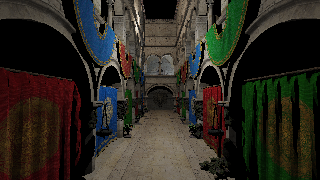
\includegraphics[width=\linewidth]{gi/temporal-static-direct.png}}{固定相机 · 三盏场景灯}
\hfill\panelimage{.318\linewidth}{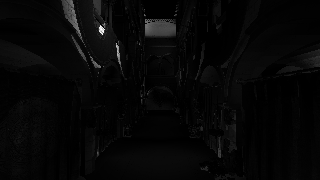
\includegraphics[width=\linewidth]{gi/temporal-ddgi-2-change.png}}{只引入低样本探针}
\hfill\panelimage{.318\linewidth}{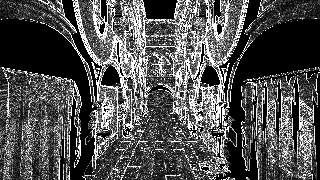
\includegraphics[width=\linewidth]{gi/temporal-direct-jitter-change.png}}{只偏移直接光采样点}
\caption{后两图比较第 23 与第 24 帧，取 RGB 三个通道中最大的显示差，再放大八倍。白色靠近变化较大的区域。右图的屋顶、布帘和纹理边缘都跟着采样位置改变。}
\end{figure}

先画逐盏计算的直接光。固定投影时，这 24 帧逐值相同；在同一个相机上只改变每帧采样点，全图有 60.89\% 的像素出现超过 3 个显示色阶的相邻帧差。这里尚未混合 TAA，测量的是它收到的输入。旧设置还把宽 320 像素的结果放大到整个面板，像素和细节一起被放大。

再固定投影，只让采样算法继续工作。将直接光和 DDGI 的一次反射相加，使用面板相同的显示曲线。每个探针方向发两条射线时，有 3.89\% 的像素变化超过同一门槛；增加到 16 条，降到 1.03\%。换成 ReSTIR GI 后为 9.31\%。单独显示 ReSTIR DI 时为 28.49\%。这些比例取第 9 至 24 帧的 15 对相邻画面，任一颜色通道从 0 至 255 的值相差超过 3 即计入一次。

这 24 帧中，每种算法记录的帧数都从 1 加到了 24，中途没有重新计数。镜头不动时，墙面仍可能因每帧只取少量光线而忽明忽暗。要检查这种抖动，可以先用面板的原始分辨率固定相机，再分别比较 TAA 混合前后的两帧。独立测试也把尺寸从 $320\times180$ 改成 $319\times179$ 再还原，逐像素核对固定相机输出和三盏灯，结果一致。

\readings{运行 \path{tests/run_gi_benchmark.cmd --temporal} 与 \path{tests/analyze_gi_temporal.py} 可重算。测量与逐帧变化图见 \path{output/profiling/gi/temporal.json} 及同目录 PNG。}

\clearpage
\fancyhead[R]{\sffamily\small\color{Muted}Vulkan / 屏幕效果实测}
\section{在屏幕上找遮挡、反射和历史}
把镜头固定在同一条走廊，一帧里先保存表面位置、法线和光照。环境遮蔽利用附近表面的高低判断这里还能看见多少天空方向；屏幕反射沿反射方向搜索另一块可见表面；时间抗锯齿（TAA）把当前像素对应的位置投回上一帧，看那时留下的颜色是否仍能使用。这三种操作读同一场景，写出的第四个数各有用途。

\begin{figure}[H]\centering
\panelimage{.318\linewidth}{
\includegraphics[width=\linewidth]{screen-effects/gtao-mask.png}}{8 · 亮处遮挡少}
\hfill\panelimage{.318\linewidth}{
\includegraphics[width=\linewidth]{screen-effects/ssr-mask.png}}{20 · 白处找到反射}
\hfill\panelimage{.318\linewidth}{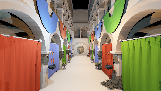
\includegraphics[width=\linewidth]{screen-effects/taa.png}}{32 · 两个采样位置的平均颜色}
\caption{遮蔽和反射两图导出第四个数，分别表示可见程度和反射射线的命中标记。右图取 TAA 的 RGB。静止相机下，回放中两次采样各占一半，可见表面的平均历史权重为 0.5。}
\end{figure}

环境遮蔽（GTAO）会沿几个屏幕方向寻找可见地平线。正常半径下，可见表面的平均可见程度为 0.899；把半径缩到 0.0001 个场景单位，平均升到 0.9997，说明原来变暗的部分来自附近的遮挡。随机屏幕反射的粗糙度取 0.08，36.34\% 的可见像素找到了画面中的反射点。固定种子重复计算得到相同颜色；粗糙度改为 0.65 后，反射方向的分布随之改变。命中率本身不能说明反射方向正确，画外和被挡住的表面也不会出现在屏幕输入里。

TAA 的对照把八个略有偏移的采样位置分别画出，保存各自的直接光，再离线取平均。相对于这份平均图，第八个单帧的均方误差为 0.001698。修正静止镜头的历史取样后，TAA 第八帧与八次取样平均仅差浮点舍入误差（$1.11\times10^{-16}$）。把镜头平移一个单位，全图约 41.0\% 的像素继续使用历史；手动重置后，全图历史权重降为零。上图捕获的是预先画过一帧、随后在未偏移镜头下再次使用历史的短序列。

\readings{八帧对照与固定种子复现见 \path{tests/ScreenEffectsTests.cpp}、
\path{tests/screen_effects_report.py} 和 \path{output/screen-effects/metrics.json}。每项算法各有一个计算着色器，文件在 \path{Renderer/ScreenSpace/Shaders/}。}

\clearpage
\section{49 盏灯怎样分配给画面}
在一条有 49 盏灯的走廊里，先把画面切成 $16\times16$ 像素的小块，再按深度分成 16 层。事件 47 为每个小空间建立灯表；事件 58 只计算表中灯的贡献。这组历史对照用四单位半径、纯漫反射和无遮挡来单测筛选。正式场景读取各点光源的半径，再检查阴影与材质高光。

\begin{figure}[H]\centering
\panelimage{.45\linewidth}{
\includegraphics[width=\linewidth]{screen-effects/clustered-mask.png}}{每个像素要检查的灯数，白色代表 49}
\hfill\panelimage{.45\linewidth}{
\includegraphics[width=\linewidth]{screen-effects/clustered.png}}{事件 58 写出的线性颜色，经曝光显示}
\caption{同一帧的两次导出。全图有 1,056 个小空间，每个用两个 32 位整数记录 49 盏灯。回放中有 627 个空间记录了编号 33 至 49 中至少一盏。}
\end{figure}

逐像素检查时，14,501 个可见像素平均访问 18.11 盏灯。用 CPU 在每个像素遍历全部 49 盏灯，两种方式得到的 RGB 最大绝对差为 $1.20\times10^{-7}$。把灯清空，输出也降为零。这里直接测到了候选数下降；要判断整帧能省多少时间，还需在相同 GPU 上对照逐灯着色与分簇两条路径，包括建立灯表的成本。

{\noindent\smalltable\begin{tabularx}{\linewidth}{@{}Xrrrr@{}}\toprule
GPU 执行内容 & 事件 & 工作组数 & 中位数（ms） & 范围（ms）\\\midrule
\screenTimingRows\bottomrule\end{tabularx}\par}

捕获来自 RTX 5070 Ti Laptop GPU，Debug/x64，分辨率 $161\times91$，右边和底边都有不完整的工作组。上表先预热一次，再以 RenderDoc 1.47 读取九轮执行时间。回放中的遮蔽、反射、分簇颜色都与独立 GPU 读回逐值相同。要比较桌面分辨率的开销，下一次应扩大视口、保持相机与灯不变，并单独测纹理读取与同步等待。

\readings{原始帧及其复现说明见 \path{output/profiling/screen-effects/}。}

\clearpage
\fancyhead[R]{\sffamily\small\color{Muted}Vulkan / 显存与光照}
\section{Sponza 的光照数据放在哪里}

在原生分辨率下观察 Sponza 中庭，显卡需要为每个像素找出射线碰到的墙面，读取材质，再结合前几帧的结果计算光照。这会反复读取三角形、用来查找三角形的包围盒树，以及保存历史颜色的数组。旧版为了让 CPU 可以直接填数组，选择了第一个允许 CPU 读写的 Vulkan 内存类型。这台笔记本上的第一个匹配项是系统内存。着色器虽然在独立显卡上运行，读取大数组时却要经过连接显卡与主机的 PCIe 总线。

本机是 NVIDIA GeForce RTX 5070 Ti Laptop GPU，驱动 616.56。驱动报告了 11.66\,GiB 的显卡本地内存和 15.90\,GiB 的系统内存。原规则选中类型 2，属于系统内存。类型 4 同时允许显卡本地读取和 CPU 映射，使用的是同一份 11.66\,GiB 的本地内存。把计算数组放到类型 4 后，加载器仍然可以把初始数据写进去。随后显卡每帧读取三角形和反复更新历史颜色时，主要使用自己的显存。

\subsection{用同一个编辑器画面比较}

两个 Debug 编辑器从相同的对象文件和引擎库链接，试验版本只替换计算数组选择的内存。打开同一份 \code{Sponza-Atrium.redflag}，固定机位，场景面板为 $1442\times964$ 像素。使用 Lit、Native、全点光源、DDGI、GTAO 和 TAA，DDGI 采样数为 2，SSR 关闭。两组都启用 Vulkan 验证层，采用同样的显示设置。打开场景后的首次模型导入与初始化不计时。每次运行再去掉 4 次预热的光照累积，统计接下来的 21 次。测量发生在静止图像停止刷新之前。

\begin{center}\smalltable
\begin{tabular}{lrrrr}
\toprule
运行次序 & 第 1 轮 & 第 2 轮 & 第 3 轮 & 第 4 轮\\
\midrule
计算数组所在位置 & 系统内存 & 本地显存 & 本地显存 & 系统内存\\
光照累积中位数（毫秒） & \memoryRunTimes\\
\bottomrule
\end{tabular}
\end{center}

把相同配置的两轮合并，各有 42 个样本。光照累积耗时的中位数从 \memoryOld\,ms 降至 \memoryNew\,ms。这个时间从 CPU 开始更新光照，到所有同步提交的 GPU 工作完成，倍率约为 $\memoryRatio$。它覆盖光照调度与等待。编辑器界面、图像呈现和其余渲染工作另行计时，因此不能把上述时间直接换算成编辑器帧率。

\clearpage
\subsection{回放同一张图，核对显卡的耗时}

为了检查显卡的工作本身有没有减少等待，用相同的 Stanford Bunny 场景各截一帧。在 $288\times192$ 下，两份 RenderDoc 帧里都有 12 次计算调度。先回放一次预热，再用 GPU 时间计数器采样 7 次，表中列出三道计算的中位数。探针更新需要查找射线打中的三角形；GTAO 则反复读取附近像素的可见表面，两者都要多次访问显存中的数组。

\begin{center}\smalltable
\begin{tabular}{lrrr}
\toprule
计算内容 & 事件编号 & 系统内存（毫秒） & 本地显存（毫秒）\\
\midrule
\memoryGpuRows
\bottomrule
\end{tabular}
\end{center}

回放脚本定位两份帧里相应事件的输出数组。DDGI、ReSTIR GI、ReSTIR DI、直接光、GTAO、屏幕反射、分簇点光和 TAA 共八张结果，每张都是四通道浮点图；逐字节对照全部一致。两份帧都没有调试消息。这组 GPU 时间只描述兔子场景的单道计算，前页的 Sponza 数据来自实际运行的编辑器。

\subsection{其他显卡怎样上传和读回}

实现位于 \code{VulkanComputeDevice::CreateBuffer}。先选择适合计算的本地显存；在最大的兼容显存堆上，优先选 CPU 能直接映射、写后双方可见的类型。只有小块显存能映射时，大数组保留在容量更大的主显存中。上传先把三角形写入暂存缓冲区，再让 GPU 复制到本地数组。读回时则由 GPU 把结果写入暂存缓冲区，待复制完成后交给 CPU。用独立测试构建强制选择本机不可映射的类型 1，三帧、35 个数组元素与 $7\times5$ 历史图均通过逐项核验。该测试检查的是这条上传和读回路径，其他型号显卡上的速度仍待实测。

\noindent\small\color{Muted}
原始 Chrome 时间线、驱动内存类型、逐帧毫秒值和 RenderDoc 回放记录位于
\path{output/profiling/compute-memory/}。对照脚本为 \path{tests/profile_compute_memory.py}。
暂存复制的接口可对照 \href{https://docs.vulkan.org/refpages/latest/refpages/source/vkCmdCopyBuffer.html}{Khronos 的 vkCmdCopyBuffer 说明}。\normalsize\color{Ink}

\clearpage
\subsection{移动相机与停手后的整帧时间}

这组历史记录测的是显存分配调整前后的编辑器，当时快速导航会切到材质底色。打开 Sponza，把场景面板调到 $948\times613$ 像素，先保持镜头不动，等面板开始沿用最后一张图。然后每隔 150\,ms 滚动一次鼠标滚轮，连续五次拉近、五次拉远，共 50 次。下表以毫秒统计完整一帧从开始到结束经过的时间，其中包含 UI、GPU 等待以及呈现。P95 表示约有 95\% 的帧在这个时间内完成。

\begin{center}\smalltable
\begin{tabular}{lrrrr}
\toprule
画面 & 旧版中位数 & 新版中位数 & 新版 P95 & 新版帧数\\
\midrule
\memoryNavigationRows
\bottomrule
\end{tabular}
\end{center}

第一行关闭“快速移动相机”。变焦过程中，显卡持续计算直接光、DDGI、GTAO 和 TAA，滚动触发的 50 个相机运动帧均进入统计。旧版同一输入只有 25 个帧观察到单独的运动，耗时较长时会在两次绘制之间收到多次滚动。第二行启用“快速移动相机”，移动过程中显示相同尺寸的材质底色图。停手后恢复完整光照并逐帧累积，缓存稳定后进入第三行。时间相近的后两行对应两种可见画面。

\begin{figure}[H]\centering
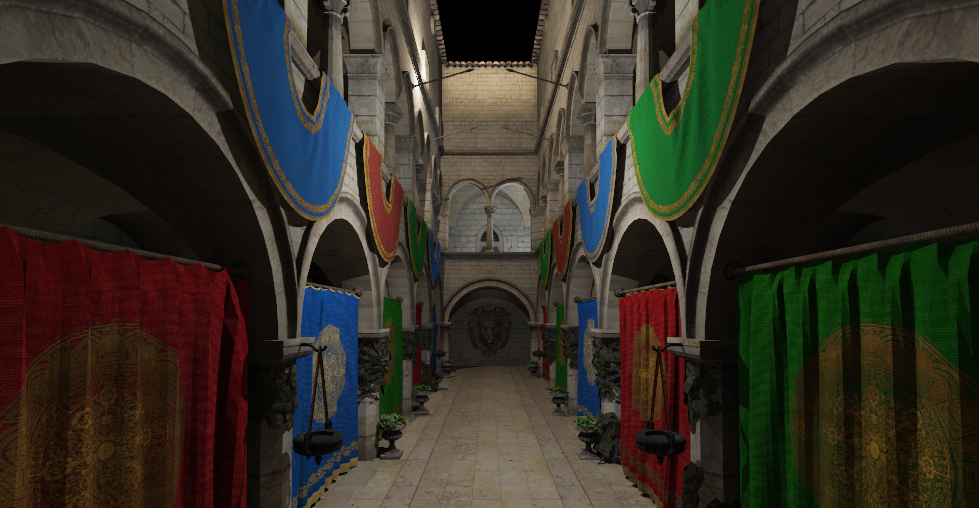
\includegraphics[width=.70\linewidth]{../editor-guide/figures/atrium.png}
\caption{正式 Vulkan 编辑器中的 Sponza 中庭，取自《编辑器使用手册》的实际视口。滚轮既改变栏杆在图上的位置，也改变为光照查找可见表面的视线。}
\end{figure}

该表用于比较新旧编辑器的整帧表现。前面只改内存分配的四轮对照则单独测量了存储数组位置的影响。同一测量目录中的 \code{final-navigation.json} 记录了每项统计，旁边保留两次正式运行的 Chrome 时间线。复现入口为 \path{tests/profile_native_navigation.py}。

\clearpage
\section{移动相机时的光照}
在 Sponza 中庭拉近镜头，观察右边挂毯上方的拱廊。默认的 Lit 视图在移动时保留完整光照。勾选「移动时仅算直接光」后，点光源仍照亮柱面，拱廊下方靠反射光照亮的区域则会变暗。停手约 0.22 秒后，编辑器重新加入 DDGI、GTAO 和 TAA，挂毯背后的暗部开始恢复。

\begin{figure}[H]\centering
\panelimage{.48\linewidth}{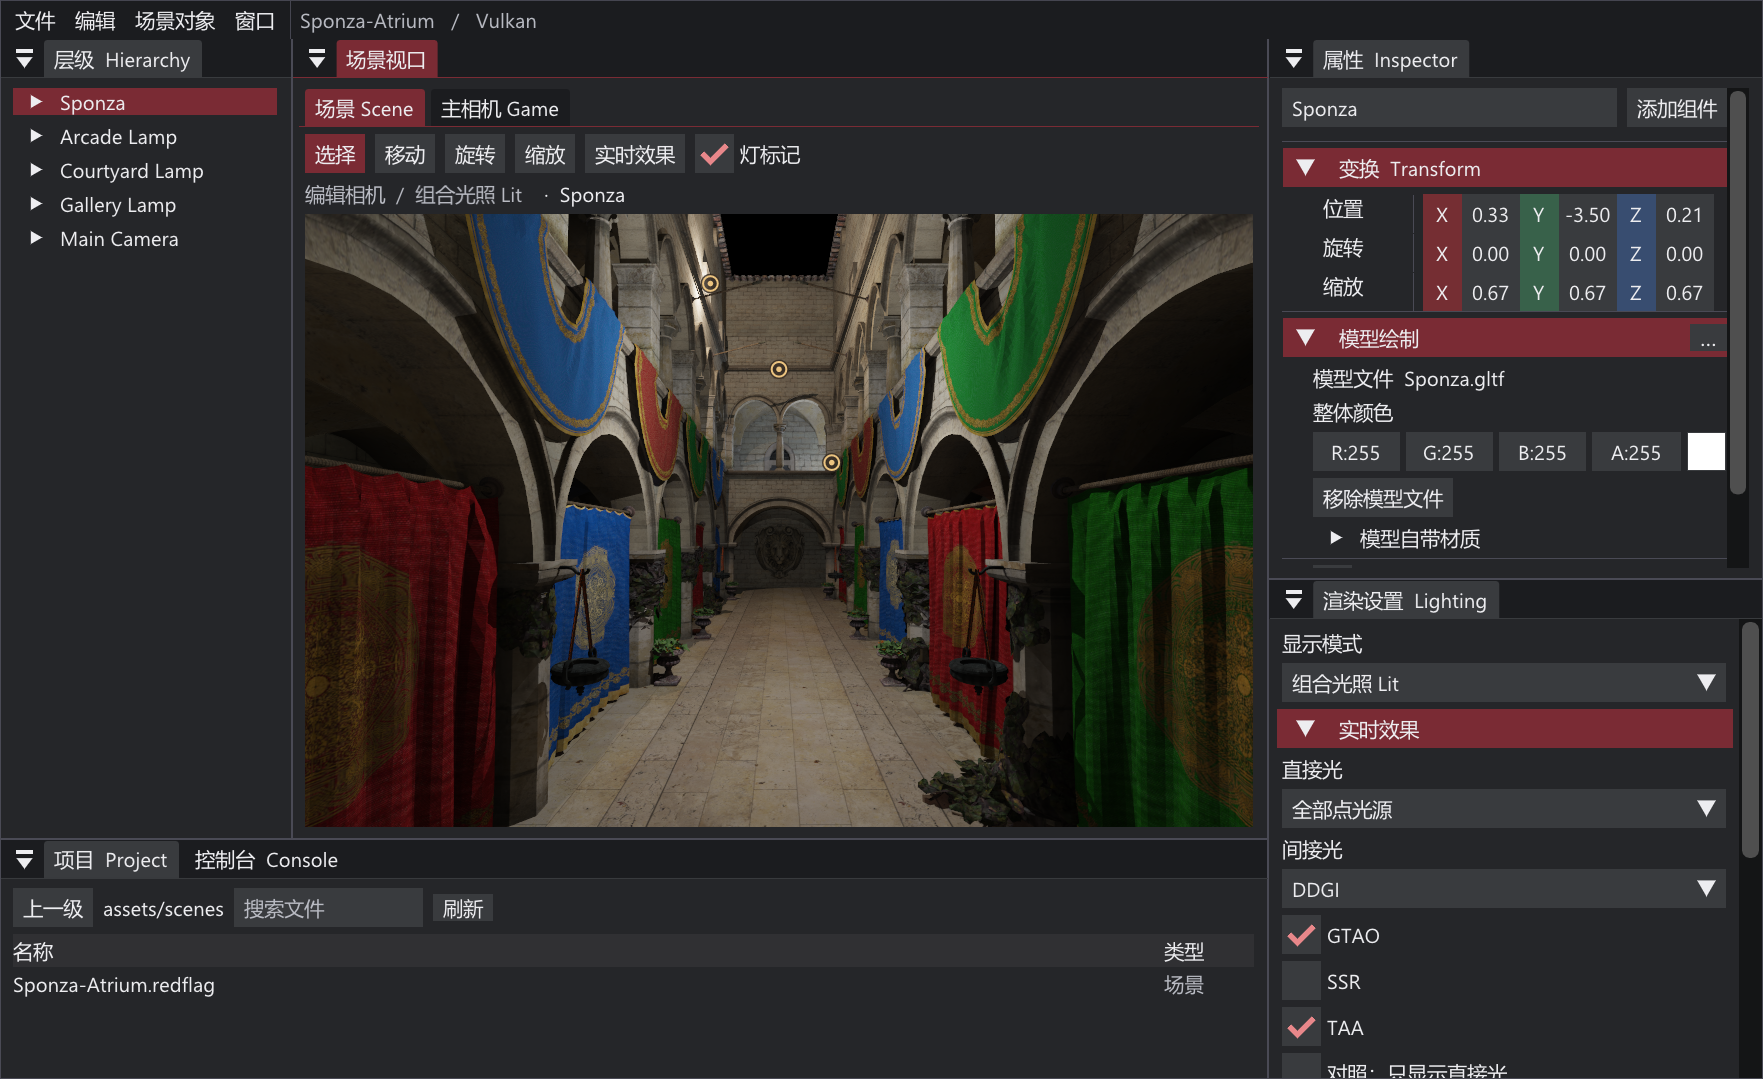
\includegraphics[width=\linewidth,trim=305bp 252bp 510bp 214bp,clip]{navigation-light/lit-motion-move.png}}{默认设置，移动中保留完整光照}
\hfill
\panelimage{.48\linewidth}{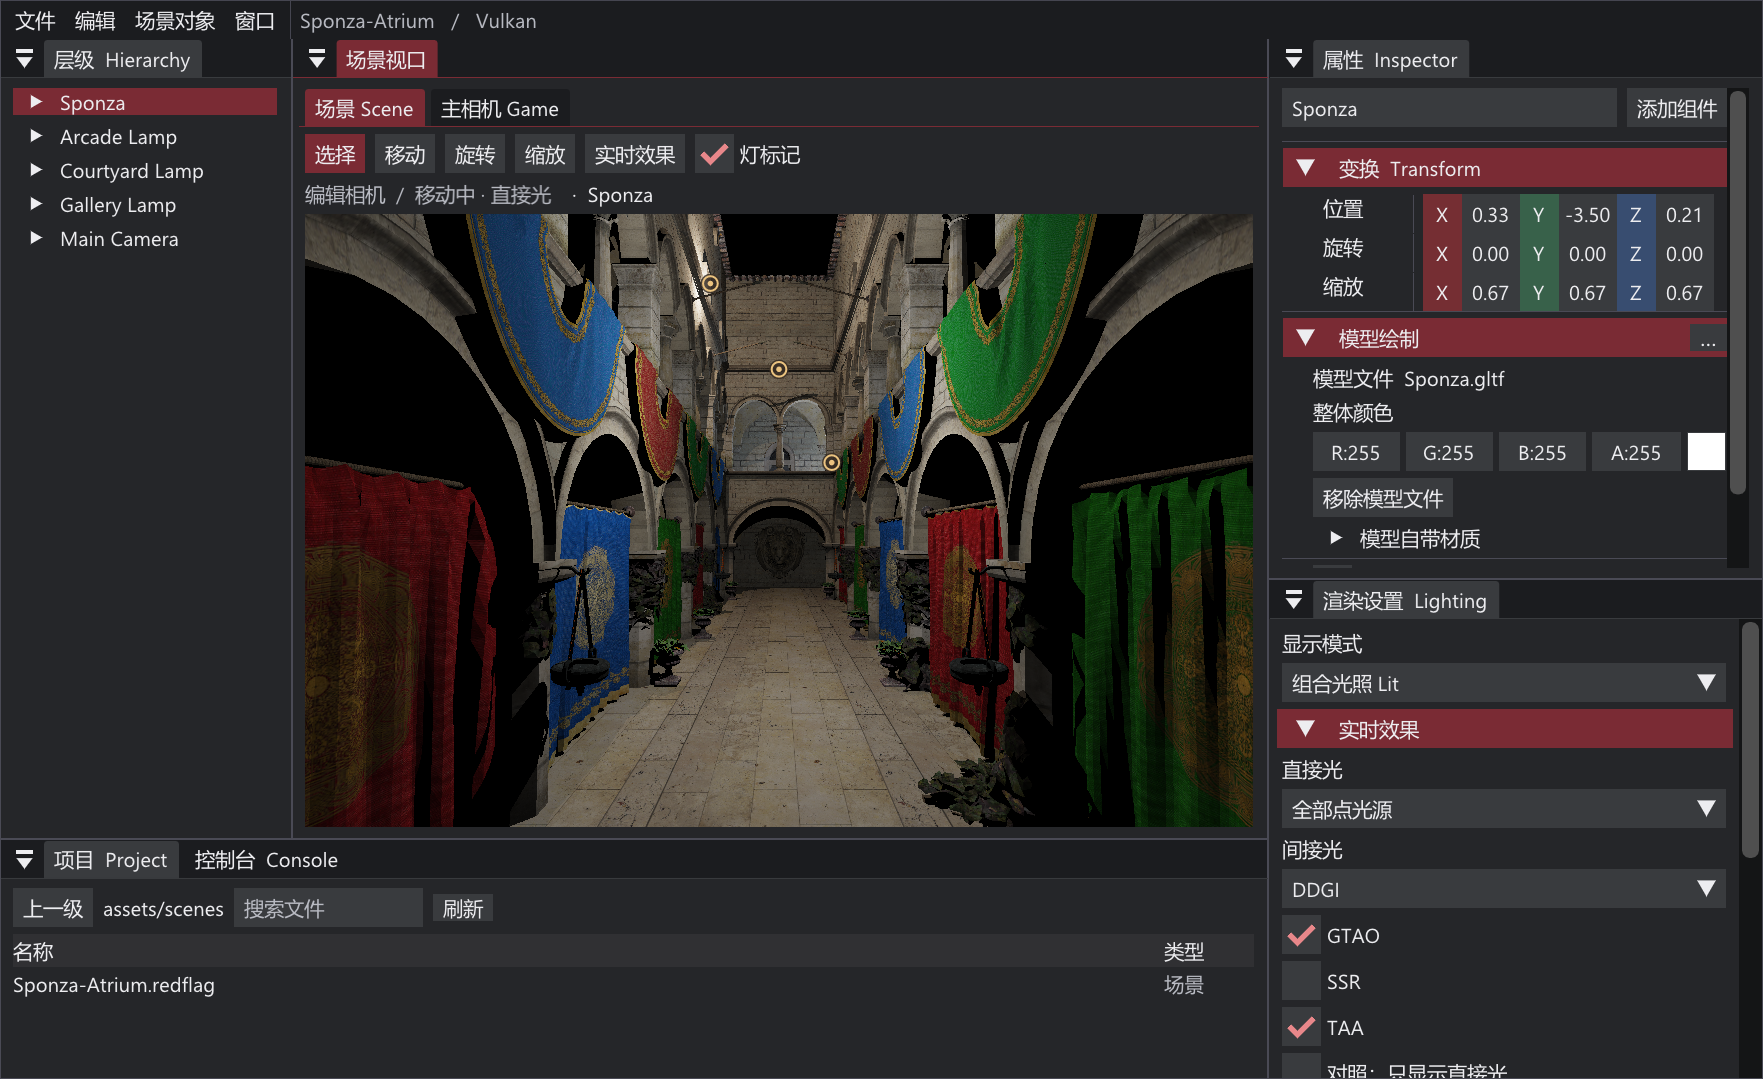
\includegraphics[width=\linewidth,trim=305bp 252bp 510bp 214bp,clip]{navigation-light/navigation-move.png}}{勾选后，同一机位只计算直接光}
\caption{两次均在计时结束后再滚动一格，约 90 毫秒后读取实际窗口，裁出相同的场景面板。两张图里挂毯的纹样和拱门的位置可以逐一对照。}
\end{figure}

关闭其他测试场景后，在同一可执行文件上各运行一次。设备为 RTX 5070 Ti Laptop GPU，Debug x64，Vulkan 验证开启。两轮都是 $948\times613$、三盏点光源、每方向两条射线的 DDGI、GTAO 与历史权重 $0.85$ 的 TAA。每隔 150 毫秒送一次滚轮输入，共 50 次。下表只取新版本中镜头实际改变并重新计算光照的帧，测量整帧经过的时间。两次输入之间直接显示缓存的帧另计。

\begin{center}\smalltable
\begin{tabular}{lrrr}\toprule
镜头改变时显示什么 & 计算帧数 & 中位数（ms） & P95（ms）\\\midrule
保留完整光照 & 50 & 15.24 & 18.62\\
只计算直接光 & 50 & 17.56 & 19.61\\\bottomrule
\end{tabular}
\end{center}

这一轮选用直接光的运动帧反而多用了约 2.3 毫秒。整帧还包含 CPU 调用、等待 GPU 和呈现，两个数不足以把差值归到某个着色器上。两次输入的间隔里，直接光可以复用已有画面。这类缓存帧的中位数是 4.06 毫秒。前页旧版底色导航的 4.15 毫秒覆盖了整个移动时段，当时画的内容和进入统计的帧都不同。

另一次在 RenderDoc 1.47 中边滚动边截取第 39 帧，面板为 $1393\times892$。事件 12 找出相机看到的表面，24 计算点光源直接照明，36 将结果写入供 ImGui 读取的图像。回放中有 103 次场景网格绘制与 22 次界面绘制。截图、事件号与两轮计时见 \path{output/profiling/navigation-light/}。镜头停下后能省去哪些计算，见第~\pageref{perf:baked-still}~页的浴室回放。

\clearpage
\section{体积雾的采样步数}
方孔左边只有一盏点光源，右边是暗室。画一个像素时，显卡把从相机到墙的路分段，逐段询问点光源能不能照到这里。光柱的边缘越窄，少量采样点越容易漏掉刚好穿过小孔的光。增加步数意味着每个像素要做更多次遮挡查询。

\begin{figure}[H]\centering
\panelimage{.48\linewidth}{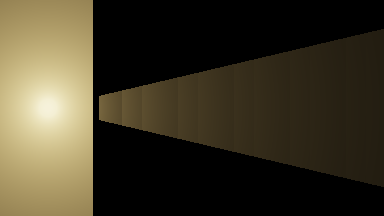
\includegraphics[width=\linewidth]{fog/open.png}}{32 步，方孔打开}
\hfill
\panelimage{.48\linewidth}{
\includegraphics[width=\linewidth]{fog/closed.png}}{32 步，只把孔封住}
\caption{Vulkan 计算结果经相同的色调映射显示。封孔后，墙右边的光束消失，左侧的灯仍照亮同一团雾。}
\end{figure}

测试固定 $384\times216$ 个像素、五个立方体组成的墙面、一盏点光源和正交相机，只改变步数。设备为 RTX 5070 Ti Laptop GPU，Debug x64，Vulkan 验证开启。每种步数预热 4 次，再单独运行 20 次。下表测的是 CPU 发出雾计算到等待 GPU 完成所经过的时间，不含模型加载、直接光、读回、窗口和 TAA。

\begin{center}\smalltable
\begin{tabular}{lrrr}\toprule
每像素的采样步数 & 8 & 16 & 32 \\\midrule
调度与等待的中位数（ms） & 0.230 & 0.327 & 0.537 \\\bottomrule
\end{tabular}
\end{center}

另一次用 RenderDoc 1.47 捕获 32 步的计算。事件 8 发出 1,296 组，每组 64 个像素，正好覆盖整幅图。预热一次后读九次 GPU 时间戳，中位数为 0.407 毫秒。回放读到像素 $(288,108)$ 的线性红色分量为 0.0227471，和普通运行一致；封孔后，该处读到 0。捕获没有报告调试消息。雾密度、相函数和遮挡的推导见《实时光照与采样》的「雾中的点光源」一章。

全分辨率的成本会随像素数、灯数和几何复杂度上升。下一次可以固定同一 Sponza 机位，比较半分辨率与全分辨率雾图，在放大半分辨率结果时参考场景深度。若光柱漏到前排石柱上，节省的时间也要和石柱轮廓附近的像素误差一起记录。

\readings{\path{tests/run_fog_tests.cmd} 可复查吸收与封孔测试；传入 RenderDoc DLL 的路径即可截帧。原始帧、采样数据及整张输出的回放摘要位于 \path{output/profiling/fog/}。}

\clearpage
\section{静态点光源的探针烘焙}

在 Sponza 走廊停下相机，用探针估计石柱上的间接光。实时版本每帧去探针位置追踪光线，再为屏幕像素插值。这组原始截帧取自单次漫反射版本，离线每方向 64 条射线，保存后下次打开场景只需插值。比较在 Debug x64 的独立 Vulkan 程序中进行，设备是 RTX 5070 Ti Laptop GPU，视口为 $160\times90$。两份实际帧只截取 DDGI 段，表面位置已在此前绘好。后来增加的多次漫反射默认烘焙四轮；这张表保留原测试条件。

{\small\noindent\begin{tabularx}{\linewidth}{@{}Xrr@{}}\toprule
操作 & 实时更新 & 读取已烘焙探针\\\midrule
探针更新，GPU 回放中位时间 & 9.369 ms & 省去\\
表面插值，GPU 回放中位时间 & 0.012 ms & 0.007 ms\\
CPU 提交到 GPU 完成，中位时间 & 10.858 ms & 0.140 ms\\
同一区间第 95 百分位 & 12.420 ms & 0.308 ms\\\bottomrule
\end{tabularx}\par}

实时组每方向取 16 个样本。RenderDoc 1.47 里，事件 8 启动 48 个工作组更新探针，事件 20 用 225 组给 14\,400 个像素插值。预烘焙组只有事件 8 的 225 个工作组。各事件的显卡时间取九次回放的中位数。插值只花几微秒，两个读数的差异很小，节省主要来自省去探针更新。

CPU 计时另开进程，顺序为实时、烘焙、烘焙、实时。每段先热身 4 次，接着记录 16 次，两组各有 32 个样本。计时区间从调用 \texttt{Render(DDGI,16)} 开始，到该调用等待显卡完成为止。打开场景、烘焙过程、直接光和界面绘制都在区间之外。这两个数字不能直接换算为编辑器帧率。重启、灯光和几何失效检查见配套光照册。

\noindent{\small 从仓库根目录执行以下两条 Windows 命令。第一条计算并保存探针，第二条启动新进程，载入后逐像素核对。}
\begin{lstlisting}
tests\run_gi_benchmark.cmd --bake
tests\run_gi_benchmark.cmd --load-bake
\end{lstlisting}

逐次数据在 \path{output/profiling/probe-bake/dispatch-and-wait.csv}。同目录 \path{renderdoc.json} 保存帧文件名、校验值、事件与九次 GPU 读数。点光源可以编辑的关卡应在布光稳定后再烘焙；需要实时移动的灯仍须重新估算间接光。后续可以逐块更新受影响的探针，用连续开关房门或移动灯具的场景检查更新时间和漏光。

\clearpage
\fancyhead[R]{\small\sffamily\color{Muted}Vulkan / 探针间的反光}
\section{探针多查一次反光的开销}
一次漫反射时，探针射线打到地板，只要算地板从点光源收到多少光。开启多次漫反射后，同一个命中点还要查询附近八个探针在上一轮记住的光。下表使用只有地面、侧墙和后墙的固定房间，直接对照这次额外查询。两次都是第四轮更新，使用同一随机种子 137，$12\times6\times7$ 个探针各有六个方向，每个方向 64 条射线，共 193,536 条。

\begin{center}\smalltable
\begin{tabular}{lrr}
\toprule
中位时间（ms）& 一次反射 & 多次反射\\
\midrule
GPU 更新探针，第 8 号事件 & 0.518 & 0.683\\
GPU 计算 $65\times65$ 画面的间接光，第 20 号事件 & 0.0068 & 0.0068\\
主线程调用两次调度并等到光照结果可用 & 0.890 & 1.022\\
\bottomrule
\end{tabular}
\end{center}

GPU 时间来自 RTX 5070 Ti Laptop GPU 上 RenderDoc 1.47 的两个真实捕获，每个先回放一次预热，再读 11 次时间戳。每份捕获都有两次计算调度、零次三角形绘制。主线程另在开启 Vulkan 验证的 Debug x64 程序中预热四次，测 11 次完整的 \code{Render} 调用，计时区间包括两个调度的录制、提交和等待。由于其中包含等待显卡的时间，不能从这一行反推驱动单独花在提交上的时间。

增加的 GPU 工作集中在探针更新。最终像素仍从同一份新探针中汇集照明，因此本例的这次调度用时相同。为了让整轮读取到相同的旧值，引擎另外保留 3,024 份方向记录，每份 32 字节，共新增 96,768 字节，约 94.5 KiB。静态多次反射要进行四轮更新，保存的文件依然只包含最后一轮。读回真实画面的对照见\href{run:Redflag-Realtime-Lighting.pdf}{《实时光照与采样》}。这组时间衡量小房间以及单项间接光；正式中庭还要另算直接光、后处理和界面。

在项目根目录执行 \path{tests/run_gi_benchmark.cmd --probe-feedback} 可重新测量主线程。若改为分批更新探针，适合在同一个机位移动点光源，记录受遮挡墙面需要几帧才恢复到新亮度，再比较节省的毫秒与多出的延迟。
\readings{\href{run:../profiling/probe-feedback/replay.json}{原始 GPU 时间与工作组数}\quad
\href{run:../profiling/probe-feedback/dispatch-and-wait.csv}{主线程逐次记录}\quad
\href{run:../profiling/probe-feedback/README.md}{源码、截图及复现方法}}

\clearpage
\section{兔子远景的网格细节}

把视口中的兔子缩小到 38 像素高，耳尖可能只占一两个像素。让显卡继续画原模型的 16\,301 个三角形，仍旧只能写进这些像素。Stanford 的原始扫描包恰好提供了同一只兔子的几份简化网格，坐标与朝向保持一致。项目选用其中三档，分别有 16\,301、3\,851 和 948 个三角形。模型从近景切换到远景时，场景中的实体、位置和覆盖材质保持一致。\href{https://graphics.stanford.edu/data/3Dscanrep/}{Stanford 模型来源}

\begin{center}
\panelimage{.43\linewidth}{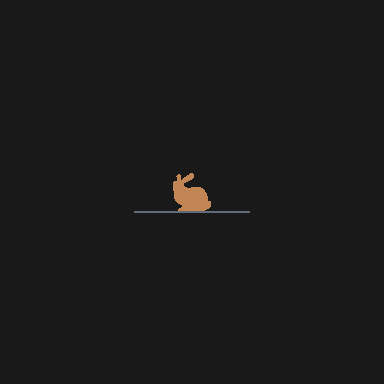
\includegraphics[width=.78\linewidth,trim=164bp 164bp 164bp 164bp,clip]{mesh-lod/Vulkan-full.png}}{LOD 0，16\,301 个三角形}
\hfill
\panelimage{.43\linewidth}{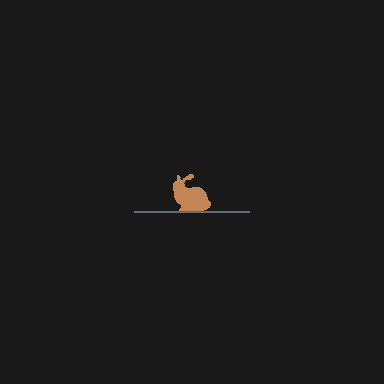
\includegraphics[width=.78\linewidth,trim=164bp 164bp 164bp 164bp,clip]{mesh-lod/Vulkan-auto.png}}{LOD 2，948 个三角形}
\end{center}
同机位的 Vulkan 基础材质实拍。原图 $384\times384$，取正中 $56\times56$ 像素放大，以便看清轮廓。耳朵和前爪仍可辨认。原网格覆盖 914 个兔子像素，简化后是 877 个；两张轮廓有 47 个像素不同，交集占并集的 94.89\%。这是此机位的取舍，模型有细长触角或镂空时，要另外检查侧面轮廓。

在层级里选中兔子，展开「属性 → 模型绘制 → 网格细节 LOD」。LOD 0 是原文件；按「添加简化模型」选择与它对齐的网格，再调「视口高度」。若使用实体的覆盖材质，各档的子网格顺序也要一致。阈值保存在场景里。示例的头两条是 25\% 与 12\%，新手可以把第一条理解为“兔子大约还占画面四分之一时换一次”。视口高 384 像素时，第一档在拉远到 $384\times0.25\times0.9=86.4$ 像素以下切换，拉近到 $384\times0.25\times1.1=105.6$ 像素以上切回。在两条线之间保留原档，轻轻来回拖相机时，耳朵就不会反复变形。

同样远的一个人和一栋楼，在屏幕上会占不同的高度。用这个比例设阈值，两件东西就能各按自己的轮廓选网格。Unity 的 LOD Group 也用对象相对于画面的高度；它可以在两档之间同时画两个模型并淡化过渡。Redflag 这里只画选中的一档，轮廓的突然变化仍要靠实际画面检查。\href{https://docs.unity3d.com/6000.0/Documentation/Manual/class-LODGroup.html}{Unity 6.0，LOD Group}

\begin{center}
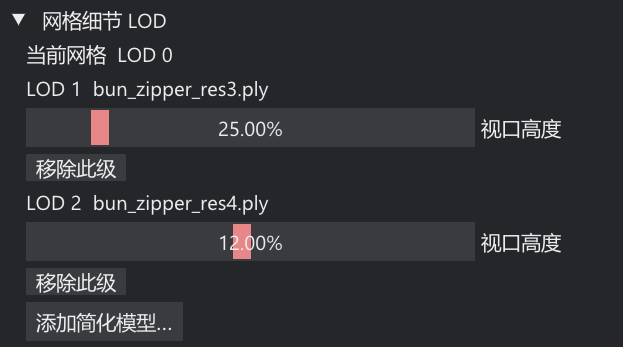
\includegraphics[width=.49\linewidth]{mesh-lod/inspector.png}\par
{\small\sffamily\color{Muted}正式编辑器的属性面板。当前用原网格，下面两行是简化模型与切换高度。}
\end{center}

\clearpage
\subsection{选定网格后的几次绘制}

导入时，\texttt{Model} 合并各部件的包围盒。绘制前，\texttt{SceneRenderer} 把原模型包围盒的八个角投影到屏幕，取最上和最下两点的高度差，得到与视口的比例。即使上一帧画了简化兔子，下一次仍用同一个原包围盒量尺寸。TAA 挪动采样位置时，选档沿用未偏移的相机。\href{run:../../Redflag/src/Redflag/Renderer/Model.cpp}{包围盒投影}\quad\href{run:../../Redflag/src/Redflag/Renderer/SceneRenderer.cpp}{场景选档和绘制}

OpenGL 场景在收集几何时选一次网格。实际截帧中，阴影、反射阴影图、深度预写和主绘制四次画兔子，远景每次都读 2\,844 个索引，保持原模型时每次读 48\,903 个。Vulkan 中，相机看到的表面、透明绘制和拾取也用同一选档。二次光线的碰撞树仍用原模型。拉远相机不会因此移动阴影遮挡物或令烘焙探针失效，但较粗的轮廓可能与精细模型投下的阴影有细微差别。

{\smalltable\noindent\begin{tabularx}{\linewidth}{@{}Xrrrr@{}}\toprule
基础材质，两次绘制（兔子与地面） & \multicolumn{2}{c}{CPU 记录两物体（微秒）}&\multicolumn{2}{c}{GPU 画兔子（微秒）}\\
\cmidrule(lr){2-3}\cmidrule(l){4-5}
后端 & 原网格 & LOD 2 & 原网格 & LOD 2\\\midrule
OpenGL & 64.40 & 52.60 & 2.400 & 0.224\\
Vulkan & 46.00 & 47.35 & 2.272 & 0.512\\\bottomrule
\end{tabularx}\par}

RTX 5070 Ti Laptop GPU、Debug x64。CPU 单独运行，每组预热四帧再记录 32 帧，表中取中位数。计时从提交场景几何开始，到记录两次绘制完成结束。每次测试都读取躯干中央的实体编号；读回在计时区间之外。GPU 时间取 RenderDoc 1.47 对同一绘制事件的九次回放中位数。三角形减少了 94.18\%，绘制调用仍是两次；Vulkan 这组 CPU 记录多用 1.35 微秒。这样的局部测量无法推算整帧能提升多少。

\noindent{\small 仓库根目录，Windows 命令。替换最后一个词为 \texttt{full}，即可用原网格作对照。}
\begin{lstlisting}
python tests/fetch_stanford.py
tests\run_mesh_lod.cmd Vulkan auto
tests\run_mesh_lod.cmd OpenGL auto
tests\run_mesh_lod.cmd OpenGLScene auto
\end{lstlisting}
各档索引数、事件编号、帧校验值和时间样本在 \path{output/profiling/mesh-lod/results.json} 与同目录的 CSV。下次可在同一位置放置多只兔子，检验几何负载增大时的整帧时间；对运动中的耳朵还可以逐帧比较档位切换前后的轮廓。

\clearpage
\fancyhead[R]{\small\sffamily\color{Muted}Vulkan / 浴室表面}
\section{浴室的第一层可见表面}
镜头对着洗手台时，一个像素究竟落在镜子、柜门还是后面的墙上？旧的 Vulkan 编辑器从相机出发，给每个像素发一条射线，在场景的三角形中找最近的交点。现在编辑器先把模型投到屏幕，深度测试留下最近的表面；同一遍绘制写出它的底色、法线和深度。现在的两份颜色输出还保存该像素的金属度与粗糙度。接着一次计算把深度还原成世界位置，仍交给原来的直接光和间接光计算。

两份真实编辑器捕获使用同一个 RTXGI 浴室、主相机、$1391\times892$ 的照明画幅，以及第 12 帧的 TAA 采样位置。旧版第 24 号事件的计算参数首项是 0，对应 \code{GI.comp} 查找第一层表面。新版有 85 次绘制，之后的第 459 号事件是 \code{PackSurfaces.comp}，把这两张输出交给后续光照。这里只计这些事件的 GPU 时间，逐次相加后再取中位数。回放一次预热，随后各测 11 次。

\begin{center}\smalltable
\begin{tabular}{lrrr}
\toprule
取得可见表面的方式 & 最短（ms）& 中位数（ms）& 最长（ms）\\
\midrule
相机射线，1 次计算 & 2.281 & 2.435 & 4.152\\
光栅化，85 次绘制＋1 次计算 & 0.375 & 0.391 & 0.752\\
\bottomrule
\end{tabular}
\end{center}

两行完成的着色细节有差别。旧版使用射线命中的三角形几何法线及缩小的贴图，光栅版本可读取材质原图和法线贴图。第二行包含把光栅结果转成表面记录的时间，其中单看第 459 号事件的中位数是 0.147 ms。每笔绘制起止之间的 GPU 时间戳没有覆盖渲染通道开始时的清图、通道结束的存储或事件间的等待。尚未测量相同输入下的 CPU 提交耗时和整帧变化。

下一次测量可以把当前分别提交的表面记录、光照和颜色合成录进同一帧的命令缓冲。已有结果说明可见表面工作本身有多长；另记 CPU 的提交与等待，才知道合并以后实际省掉多少。继续使用这个机位，分别统计静止 32 帧和镜头移动期间的帧时间。

\readings{\href{run:../profiling/primary-surfaces/summary.json}{原始毫秒、文件哈希与事件}\quad
\href{run:../profiling/primary-surfaces/README.md}{RenderDoc 环境与复测命令}\quad
\href{run:Redflag-Source-Guide.pdf}{源码读本 · 石柱的表面与光照}}

\clearpage
\fancyhead[R]{\sffamily\small\color{Muted}一帧的组织与诊断}
\section{场景、绘制命令与渲染线程}

神庙的长廊里有多件共用石材的模型。改动一盏灯时，可以继续使用石柱的网格和纹理。相机看到哪一面、石柱在新灯光下有多亮，则需要重新计算。Redflag 把能长期保存的材质、网格和纹理与本次绘制需要的位置、相机和目标图分开。这样就能单独检查一次材料导入，或一帧中的一次着色。

\begin{figure}[H]\centering
\panelimage{.315\linewidth}{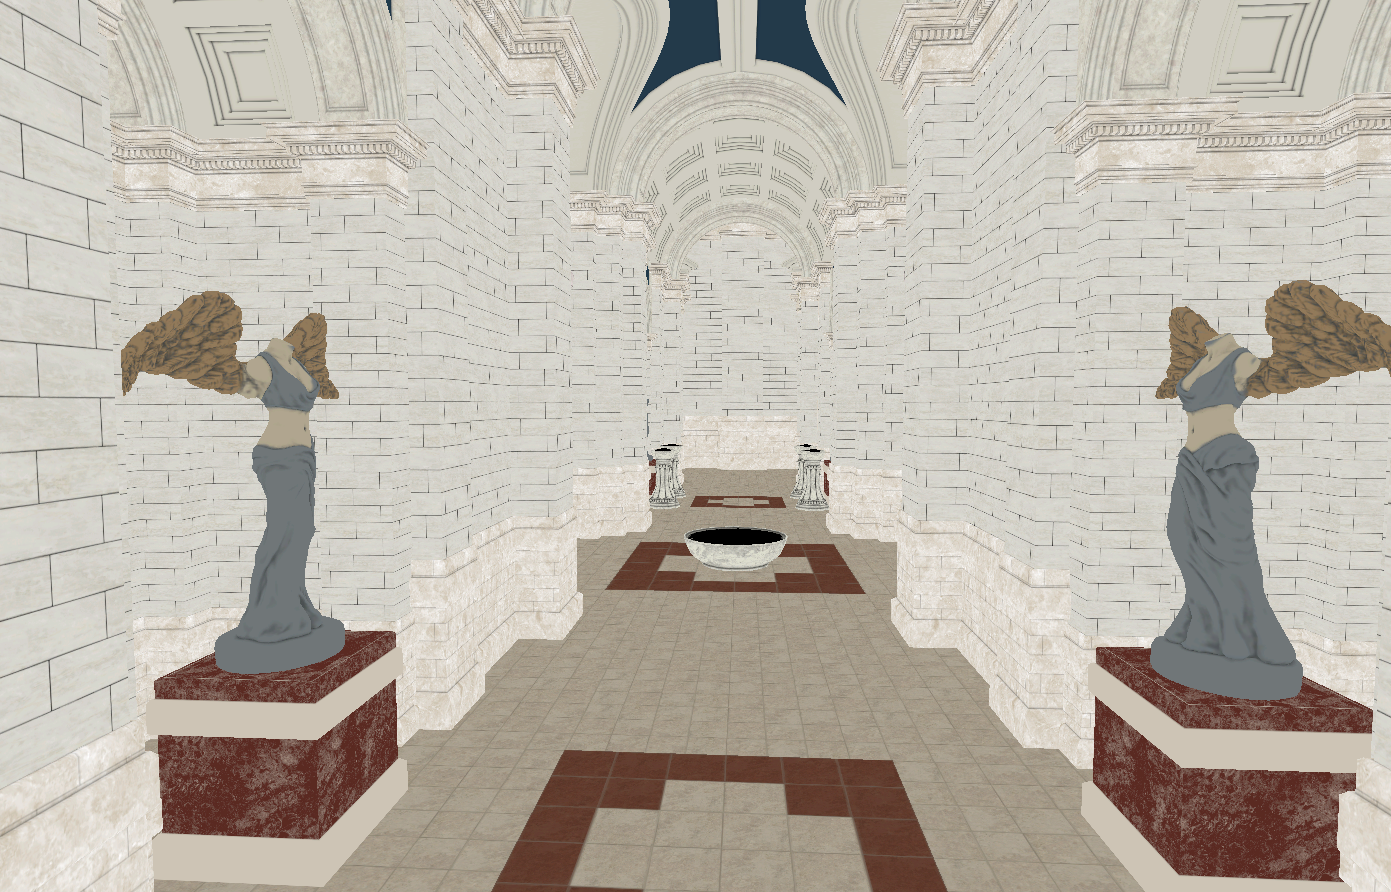
\includegraphics[width=\linewidth]{../../../output/scenes/sun-temple/albedo.png}}{材质底色}
\hfill
\panelimage{.315\linewidth}{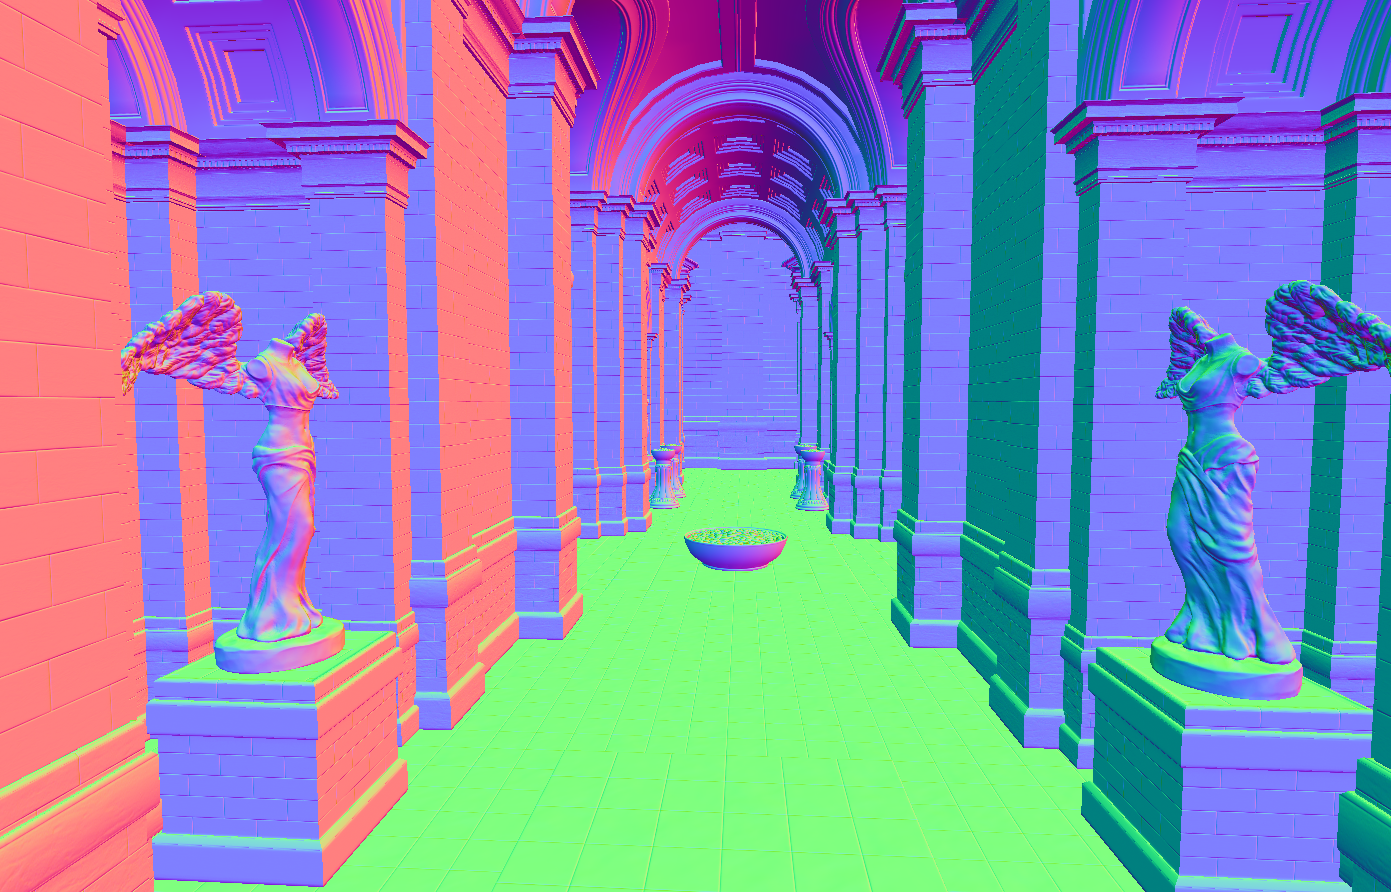
\includegraphics[width=\linewidth]{../../../output/scenes/sun-temple/normal-depth.png}}{表面朝向}
\hfill
\panelimage{.315\linewidth}{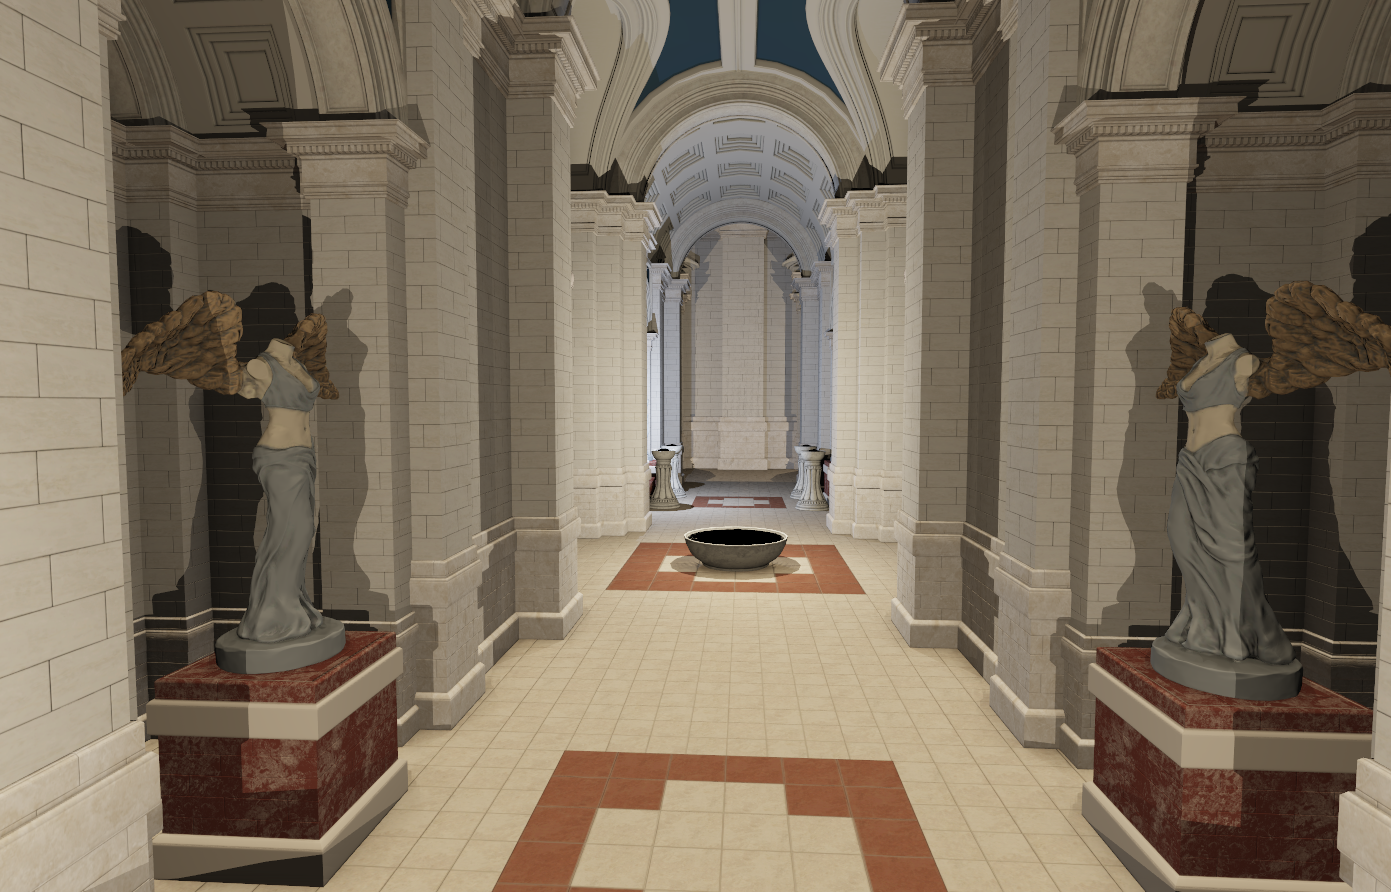
\includegraphics[width=\linewidth]{../../../output/scenes/sun-temple/SunTemple.png}}{编辑器场景颜色}
\caption{Vulkan 编辑器中的同一处神庙。左图能检查纹理是否贴对，中央能检查石柱的轮廓和朝向，右图才把光照加进来。场景由 Epic Games 制作，经 NVIDIA ORCA 发布，CC BY-NC-SA 4.0。}
\end{figure}

\code{Application::Run} 在应用主循环中更新各层，再调用它们的界面绘制。场景和编辑器选择相机、实体、子网格和材质。到 \code{VulkanDraw::DrawIndexed} 时，这些选择已经完成。后端绑定这份网格的顶点和索引，把这次的位置和编号写入命令，再调用 \code{vkCmdDrawIndexed}。这条 draw call 告诉 GPU 从索引中取出哪些三角形。提交命令后，CPU 能继续执行，GPU 在自己的队列上处理绘制。后端按帧保留所用网格和贴图的引用，等这一帧的完成信号（fence）到了，才可以重用该帧的位置、释放这些引用。

UE 的 Game Thread 更新游戏对象，Render Thread 在另一个 CPU 线程上准备渲染。Epic 举的例子是角色组件和它的渲染代理：渲染线程用自己的数据副本，游戏线程可以继续改角色。Redflag 此处沿主循环直接调用后端。若以后把准备命令移到单独线程，先把本帧的变换、材质引用和实体编号固定下来，再交给另一线程。仅把函数放入线程池，会让它读到下一帧甚至已被删除的实体。\source{https://dev.epicgames.com/documentation/en-us/unreal-engine/threaded-rendering-in-unreal-engine}{Epic · Threaded Rendering}

\readings{调用入口见 \path{Redflag/src/Redflag/Core/Application.cpp} 与 \path{Redflag/src/Platform/Vulkan/VulkanDraw.cpp}。神庙的逐事件记录与原始资源许可见 \path{output/scenes/sun-temple/README.md}。}

\clearpage
\section{阶段之间传递的图像}

先看直接光与间接光合成的那一步。直接光是灯直接照到石柱的部分，间接光来自其他表面的反射。GTAO 根据附近的遮挡给出一个零到一的数，放在遮蔽图的透明度通道。下列代码保留直接光，在开关启用时用遮蔽值减弱间接光；同一像素的两部分随后相加。颜色直到显示阶段才转换到屏幕使用的范围。
\begin{lstlisting}
// 只给间接光乘遮蔽。最后加回直接光，写出本像素的线性颜色。
vec3 reflected = hasIndirect != 0 ? indirect[i].rgb : vec3(0);
if (useAO != 0) reflected *= occlusion[i].a;
combined[i] = vec4(direct[i].rgb + reflected, 1);
\end{lstlisting}
{\small\path{RedflagForge/src/Shaders/CombineLight.comp}\quad 计算着色器 \code{main}}\par

\code{LightingPreview::RenderLit} 用普通函数明确排好这几步。选择灯光算法后，先生成直接光和可选的间接光，再合成颜色。SSR 读合成后的场景找倒影。雾要用视线的终点和灯光遮挡，TAA 还要用上一帧留下的结果。关闭一个效果时，把已有的颜色直接传给下一步。选择只看直接光时，算完直接光就可以返回。

UE 的 Render Dependency Graph（RDG）让各阶段先声明自己读写的资源。以同一张合成颜色图为例，图中会有“合成写入，SSR 读取”这条依赖。知道最后一个读者是谁，执行器才有机会回收占用的内存，或在合适的位置安排 GPU 同步。项目当前把顺序和图像保存在 C++ 对象里。固定顺序很容易沿源码检查；将来若多种画法都需要自行判断一张图何时能复用，优先把它们共用的颜色、深度及历史图的读写记录下来，再考虑自动安排。\source{https://dev.epicgames.com/documentation/en-us/unreal-engine/render-dependency-graph-in-unreal-engine}{Epic · Render Dependency Graph}

从一个数据结构就能估显存量级。每个合成像素是一个 \code{vec4}，四个 32 位浮点数占 16 字节。在 $948\times613$ 的面板上，单份颜色数组的数据占 $948\times613\times16=9{,}297{,}984$ 字节，约 8.87 MiB。此前把光照数组换到显卡本地内存，实测 Sponza 的光照更新从 \memoryOld\,ms 变为 \memoryNew\,ms。数组尺寸保持原样，变化在于 GPU 从哪里读它。报告显存节约还需要统计同时存活的所有分配、驱动对齐和峰值；报告帧率则应计完整呈现帧。

\readings{实际输入与输出见 \path{RedflagForge/src/Shaders/CombineLight.comp}，调用与生成数组的位置见 \path{RedflagForge/src/LightingPreview.cpp}。前文「Sponza 的光照数据放在哪里」保留设备、尺寸与逐次计时。}

\clearpage
\section{从一次慢帧定位到具体工作}

64 个不重叠的方块提供了一个可复查的反例。先做深度预写（Pre-Z），GPU 能预先知道每个像素离相机最近的表面。若后面的几何被它挡住，硬件有机会在执行昂贵的片元着色之前就丢弃这些片元，这叫提前深度测试（Early-Z）。不同三角形覆盖同一像素叫重复覆盖（overdraw）。本次方块相互错开，RenderDoc 回放中开关预写，主绘制的片元着色调用都是 43,264 次。打开预写还多了 64 次绘制，GPU 区间中位数从 6.912 增至 9.248 微秒。换成前后重叠的墙面，才值得重新测量它能否减少整帧工作。

同一份深度也能帮忙排错。树叶常画在矩形上，材质用贴图的透明度裁掉空白。曾经主绘制留下孔洞，深度预写却把孔洞也填上，后面的物体便消失了。调试时先看预写结束那一刻的深度，再找叶片着色器用哪张图判断透明。修复让两个阶段使用相同的底色透明度和裁剪阈值。项目用 1,024 个像素逐点比较深度；和主绘制结果相同后，才把问题归到已修复。详见《渲染排错记录》的深度预写实测。

若慢的是合成或光照计算，先定位到具体 dispatch，再改变单一条件。读相邻像素时，临近地址的数据可能已在缓存（cache）里，GPU 便能少从显存取一次。显存带宽是每秒实际传输了多少字节；数组大小乘帧率只能估算数据量。GPU 还把多条线程组成一组来发射指令，这种执行方式叫 SIMT。在 NVIDIA 硬件上，一个 warp 有 32 条线程。如果同组的一些线程沿光线很快遇墙、另一些要走很远，执行不同分支时就可能有一部分线程空等。一次 dispatch 的耗时同时受这些因素影响。

实际排查可以固定灯和相机，先比较相同画面的 CPU 提交与 GPU 时间戳；若 GPU 的某一阶段明显较长，再改变分辨率或每条光线的采样数。当前项目的逐事件和像素证据来自 RenderDoc，区间耗时另由 GPU 查询或独立运行记录。要判断是显存带宽接近上限、缓存命中偏低，还是线程利用率低，可以在 NVIDIA 上针对这个区间再采 Nsight Graphics 的 GPU Trace。PIX 的 GPU Capture 面向 Direct3D 12，可用于对照该后端的事件和计数。此处未采集 Nsight 或 PIX 的硬件计数。

\readings{\path{output/profiling/mesh/replay.json} 记录 Pre-Z 事件，\path{output/profiling/mesh/timing.csv} 保留原始计时。参见 \refitem{https://docs.nvidia.com/nsight-graphics/UserGuide/gpu-trace-overview.html}{Nsight Graphics GPU Trace}、\refitem{https://docs.nvidia.com/cuda/cuda-c-programming-guide/index.html}{NVIDIA 的 SIMT 与 warp 说明}及 \refitem{https://learn.microsoft.com/en-us/windows/pix/gpu-captures/gpu-captures-overview}{Microsoft PIX GPU Capture}。}

\clearpage
\fancyhead[R]{\sffamily\small\color{Muted}Vulkan / 点光源与材质}
\section{带材质的逐灯与分簇绘制}

把三盏灯放在一块橙色金属板前，灯的半径依次取 6、4 和 3 个场景单位。这次先让每个像素按顺序检查三盏灯，再让分簇算法先查灯表。两边都从同一个点向灯检查遮挡，并读取同一份粗糙度、金属度。把板子换成粗糙金属或非金属后，双精度 CPU 程序仍可逐灯给出参照。CPU 采用 glTF 附录 B 的反射公式，独立计算表面能反进眼睛的亮度。

{\smalltable\noindent\begin{tabularx}{\linewidth}{@{}Xrrrr@{}}\toprule
橙色面板 & 中心红通道 & 分簇与逐灯最大差 & 单帧 MSE & 64 帧均值 MSE\\\midrule
非金属，粗糙度 0.25 & 1.170 & 0.0000725 & 0.01088 & 0.000396\\
金属，粗糙度 0.70 & 0.346 & 0.00000039 & 0.00416 & 0.000199\\
金属，粗糙度 0.25 & 16.105 & 0.000565 & 0.31989 & 0.004313\\\bottomrule
\end{tabularx}\par}

最大差取整幅 $33\times33$ 图像、三个线性 RGB 通道中的最大绝对值。后两列以 CPU 逐灯解为参考，比较一次 ReSTIR DI 输出，以及连续 64 帧的平均。中心高光最窄的那块面板，抽到正对镜头的灯与抽到侧灯会得到很不一样的亮度，因此单帧误差最大。这个场景检验了把材质高光计入选择权重后，增加样本能否让整张图接近参照。

RTX 5070 Ti Laptop GPU，Vulkan Debug x64。RenderDoc 1.47 的事件 8 逐灯绘制，22 建灯表，33 使用灯表绘制。对同一帧先预热一次、再回放 11 次，三步 GPU 时间中位数依次为 4.608、3.264、4.576 微秒。分簇的两步合计约 7.84 微秒，在三盏灯的小图上，建表已比它省下的着色工作耗时更长。增加灯数和画幅后需重测。

另起未挂 RenderDoc 的进程，两种方法交替先执行，预热四组后再各记 21 组。从发起计算到主线程等到结束，逐灯和分簇的中位数是 151.3 与 242.4 微秒。这段还包含命令提交、驱动与等待，不能作为纯 CPU 录制耗时。两光路有相同的阴影测试；实际放入一块完全遮住点光源的立方体时，板中心两处读数都为零。

\begin{figure}[H]\centering
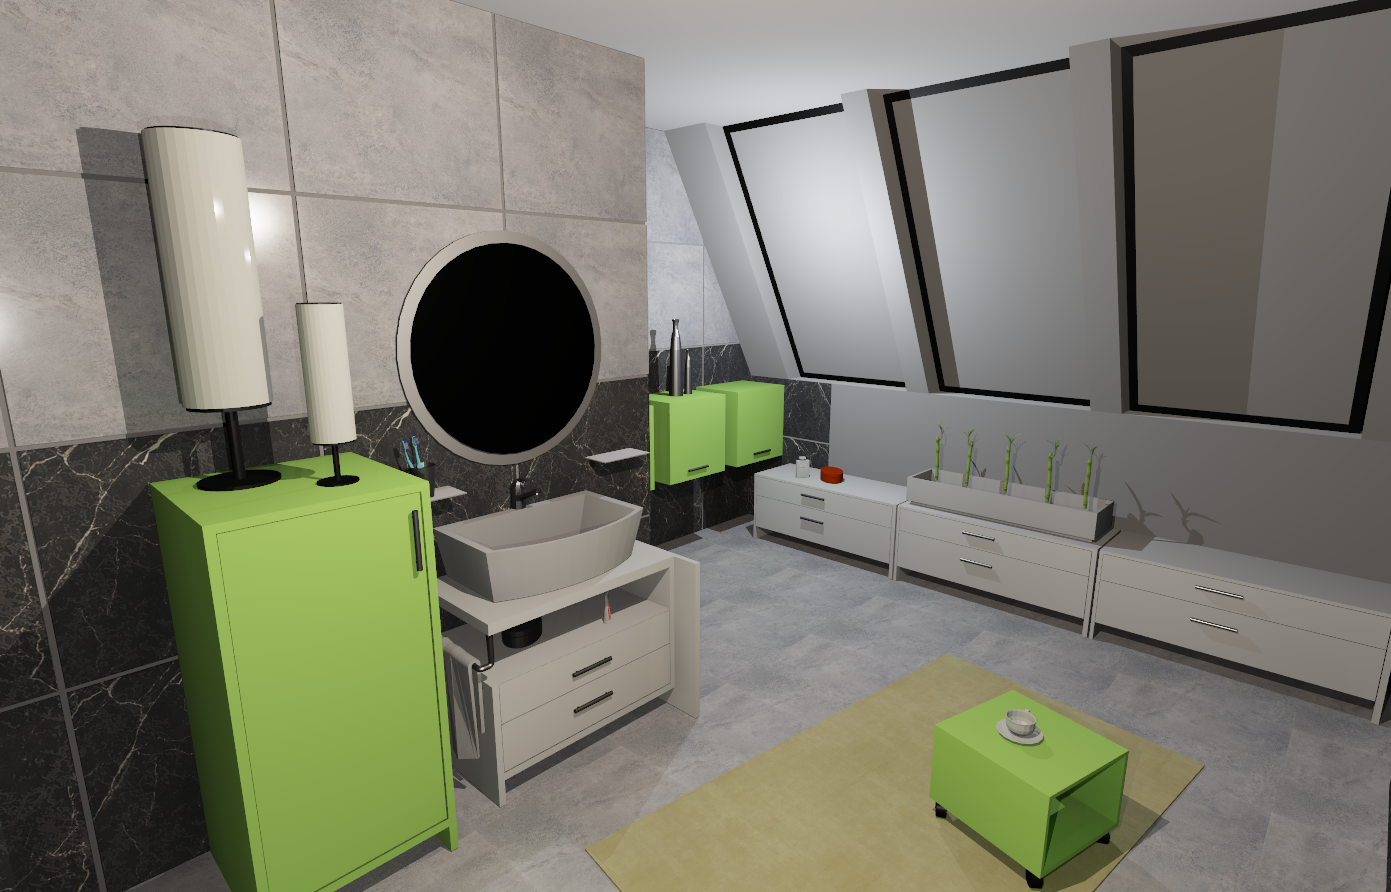
\includegraphics[width=.69\linewidth]{point-materials/bathroom-pbr.png}
\caption{把同一着色公式用到浴室的灯壳和柜门。实际编辑器重新打开已烘焙的场景，RenderDoc 第 12 帧，场景面板原图为 $1391\times892$。上表的计时取自三灯面板测试。}
\end{figure}

\readings{\href{run:../profiling/point-materials/renderdoc.json}{帧号、事件、全部 GPU 计时}\quad
\href{run:../profiling/point-materials/point-times.csv}{主线程计时}\quad
\href{run:../profiling/point-materials/point-materials.csv}{材质与误差}\quad
\href{run:../profiling/point-materials/README.md}{源码与复现方法}}

\clearpage
\section{远处地面的纹理闪动}
\label{sec:texture-minification}
\fancypagestyle{miptexture}{\fancyhead[R]{\sffamily\small\color{Muted}Vulkan / 纹理过滤}}
\thispagestyle{miptexture}

一黑一白的细格铺在地面上。走近能分辨格子，远处一个像素可能盖住几十格，应该看到稳定的灰色。旧版 Vulkan 只上传最大的那张贴图。相机略微向右移动，屏幕像素就会从黑格滑到白格，地面出现了原图中没有的明暗条纹。

\begin{figure}[H]
\centering
\begin{tabular}{@{}ccc@{}}
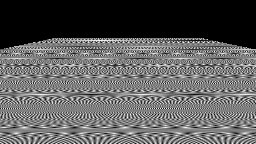
\includegraphics[width=.31\linewidth]{../../../output/profiling/texture-minification/old/frame-b.png} &
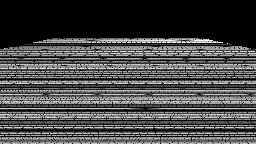
\includegraphics[width=.31\linewidth]{../../../output/profiling/texture-minification/old/motion-x4.png} &

\includegraphics[width=.31\linewidth]{../../../output/profiling/texture-minification/fixed/frame-b.png} \\
{\small 单层贴图} & {\small 旧版两帧的差异} & {\small 修复后的地面}
\end{tabular}
\caption{中图将相机移动前后两张显示图逐像素相减，绝对差放大四倍。地面内部越亮，说明这里闪动越明显。左右图的机位、贴图和曝光一致。}\end{figure}

相机横移 0.007 个场景单位，中央参照点在 $256\times144$ 的画面上只走了 0.206 像素。测试直接读底色，关掉灯光和 TAA，对地面内部相同的 8,256 个像素求两帧线性亮度的平均绝对差。单层贴图读到 $0.09129$；补齐逐级减半的九层贴图后，这组像素的差降到 0。黑白各半的正确亮度是 0.5，第二帧的均值由 0.24262 变为 0.50391。缩图使用 8 位存储，加上纹理单元的采样精度，结果与 0.5 略有距离。

底色图中的字节表达显示用的 sRGB 颜色。显卡在生成缩图、绘制时都先把它们换成线性亮度再过滤。粗糙度等数据直接按数值取平均，透明度也如此。两份 RenderDoc 截帧的地面绘制都在事件 11。黑白格第一次缩小后，底色图灰度字节是 188，数据图是 127。用户把同一张图交给这两种用途时，引擎才各留一份；屏幕上的场景面板仍然只有一层。

RTX 5070 Ti Laptop 的驱动为旧 $256^2$ 贴图要求 262,144 字节显存，新的一条链占 351,232 字节，增加 87 KiB（约 34\%）。此例刻意把一张图同时作底色和材质数据，两条链共 702,464 字节。单用途贴图只付一条链的费用。设置透明阈值 0.5 后，底色的 Alpha 和独立透明图分别用 127 与 128 两个字节验证；左半边均露出背景，拾取为 $-1$，右半边仍是实体 7。

\note{Debug/x64，\path{tests/run_texture_minification.cmd}；两份截帧、原图与显存读数在 \path{output/profiling/texture-minification/}。层级生成见 \path{VulkanDrawResources.cpp} 的 \code{BuildMips}，材质采样见 \path{Platform/Vulkan/Shaders/Mesh.frag}。}

\clearpage
\fancyhead[R]{\sffamily\small\color{Muted}Vulkan / 场景面板}
\section{浴室光照的重复计算}
\label{perf:baked-still}
\begingroup
\setlength{\parindent}{2\ccwd}
打开 RTXGI Bathroom，镜头对着洗手盆和圆镜。房间里各处接到的反射光已经保存在探针文件中。镜头和灯都没动，从同一组探针给同一片墙取光，两次算出的颜色会一样。旧版在面板大小稳定后还连续算了 32 帧。新版画好第一帧就把这张图留给界面。

\begin{figure}[H]\centering
\begin{minipage}[c]{.42\linewidth}\centering
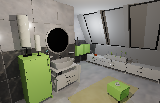
\includegraphics[width=.96\linewidth]{navigation-light/baked/after.png}
\end{minipage}\hfill
\begin{minipage}[c]{.55\linewidth}\centering
{\smalltable\begin{tabular}{@{}lrr@{}}\toprule
第 24 帧的 GPU 调用 & 旧版 & 新版\\\midrule
计算光照和面板颜色 & 4 & 0\\
绘制场景网格 & 85 & 85\\
绘制编辑器界面 & 22 & 22\\\bottomrule
\end{tabular}}
\end{minipage}
\caption{左图从新版事件 510 读取，当时 ImGui 正在显示这张浴室贴图。旧版事件 558 读到的也是这幅图。两份原图均为 $160\times103$，表中每一项按实际 GPU 命令计数。}
\end{figure}

两版均用全部点光源加上烘焙 DDGI。关闭 TAA、GTAO、SSR 和快速导航后，以同一机位运行正式 Vulkan 编辑器。旧版在事件 11 计算直接光，23 读取烘焙探针给表面补光，35 将两者相加，47 把颜色写进面板图。新版直接让 ImGui 读已经画好的贴图。用于鼠标拾取的物体编号仍随场景网格绘制，界面也照常响应。

\begin{figure}[H]\centering
\begin{tikzpicture}[x=1.98mm,y=1mm,font=\sffamily\footnotesize]
  \fill[Rust] (9,14) rectangle (11,18); \node[right] at (11.8,16){重新计算光照};
  \fill[Teal!40] (32,14) rectangle (34,18); \node[right] at (34.8,16){沿用面板图};
  \foreach \row/\limit/\labelname in {8/32/旧版,1/1/新版}{
    \node[left] at (-1,\row) {\labelname};
    \foreach \i in {1,...,55}{
      \ifnum\i>\limit\relax\def\cellcolor{Teal!40}\else\def\cellcolor{Rust}\fi
      \fill[\cellcolor] (\i-1,\row-1.85) rectangle (\i-.10,\row+1.85);
    }
  }
\end{tikzpicture}
\caption{每格是面板大小稳定后的一帧，从左往右共 55 帧。旧版前 32 帧计算光照，随后 23 帧沿用原图；新版计算 1 帧，余下 54 帧沿用原图。}
\end{figure}

直接对照 ImGui 收到的浮点纹理，16\,480 个像素的红、绿、蓝和透明度逐字节相同。打开 TAA 后，镜头虽然不动，每帧仍会在像素内换个位置取样；另一轮 48 帧的检查中，新版为此保留了 32 帧计算。两份捕获来自 RTX 5070 Ti Laptop GPU、Debug x64、RenderDoc 1.47。这次测的是调用次数与画面，整帧耗时需另作计时。

{\small\color{Muted}截图、两份原帧的校验值及复查命令见 \path{output/profiling/navigation-light/baked/}。\par}
\endgroup

\clearpage
\fancyhead[R]{\sffamily\small\color{Muted}Vulkan / 材质发光}
\section{火盆的自发光绘制}
Sun Temple 中央的火盆只占画面一小块。初版为了算出哪些炭火能被相机看见，又画了一遍房间里的全部网格。其实主绘制已经留下了离相机最近的表面深度。再画火盆时，只要它在某个像素的深度等于已存深度，这个像素就有机会发光；挡在前面的柱子已经决定了遮挡，无需重画。

\begin{figure}[H]\centering
\begin{minipage}[c]{.635\linewidth}\centering
\begin{tikzpicture}
\node[anchor=south west,inner sep=0] (photo) at (0,0) {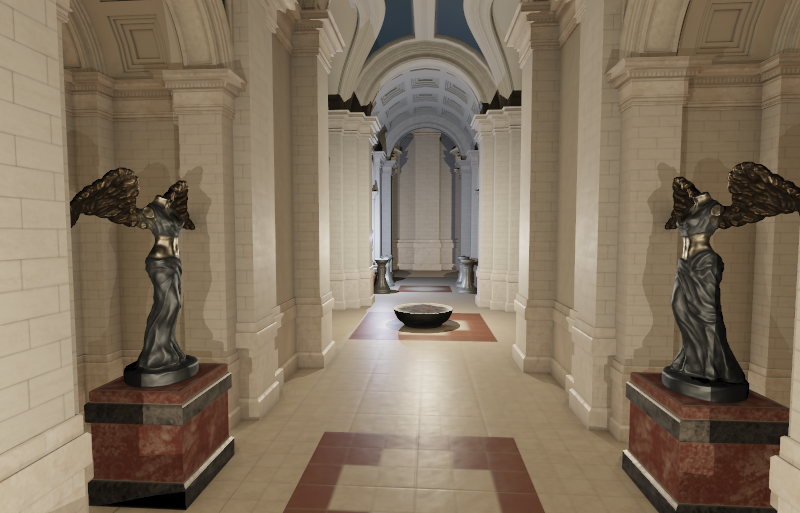
\includegraphics[width=\linewidth]{emissive-material/temple.png}};
\begin{scope}[x={(photo.south east)},y={(photo.north west)}]
\draw[white,line width=1.4pt] (.43125,.31774) rectangle (.59875,.54386);
\draw[Rust,line width=.65pt] (.43125,.31774) rectangle (.59875,.54386);
\end{scope}
\end{tikzpicture}
\end{minipage}\hfill
\begin{minipage}[c]{.32\linewidth}\centering
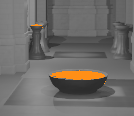
\includegraphics[width=\linewidth]{emissive-material/temple-emission.png}
\end{minipage}
\caption{左图是正式编辑器第 24 帧的面板颜色。右图放大方框，橙色标出回放中发光值大于零的 396 个像素，灰色保留火盆的轮廓。两版全部 410\,400 个像素的线性光照与显示颜色分别逐字节相同。}
\end{figure}

{\smalltable\noindent\begin{tabularx}{\linewidth}{@{}Xrr@{}}\toprule
同一帧的工作 & 重画全部网格 & 沿用主表面深度\\\midrule
发光绘制次数 & 48 & 4\\
这些绘制读取的索引数 & 1\,819\,128 & 202\,122\\
发光绘制的 GPU 时间（微秒） & 169.73 & 16.83\\
将发光加入场景的 GPU 时间（微秒） & 10.75 & 16.29\\\bottomrule
\end{tabularx}\par}

新版只提交四个发光网格。两片材质若恰好共面，光凭深度无法分出先后。主绘制把胜出的材质是否发光记在底色图里，合成时多读一次这个标记，因此表中最后一项稍慢。两版均保留 48 次主表面绘制、48 次拾取绘制与 22 次界面绘制。宽高为 $800\times513$ 时，发光图和合成结果合计 12.52\,MiB。沿用深度可少存一张 D32 图，省去 1.57\,MiB 像素数据；这里按格式计算，驱动分配对齐另计。

设备是 RTX 5070 Ti Laptop GPU，Debug x64，Vulkan 验证开启。每份 RenderDoc 1.47 捕获先回放一次，再测 11 次，表中为中位数。两版模型顶点因新增发光 UV 从 44 增至 52 字节。CPU 在这一次捕获中进入各条 \code{vkCmdDrawIndexed} 的耗时之和为 121 与 32 微秒，其中包括截帧开销。另用没有发光材质的古董相机复查，两个版本均为 29 次绘制、9 次计算，颜色逐像素相同。

{\small\color{Muted}原帧、逐次读数和复查命令见 \path{output/profiling/emissive-material/}。\par}

\clearpage
\fancyhead[R]{\sffamily\small\color{Muted}Vulkan / 阴影与探针}
\section{三角形的共边与光照耗时}
神庙的墙由许多三角形拼成。一条光线正好打在两个三角形共用的边上，如果两边都判定光线落在自己外面，光线就会穿过墙。用前后紧挨的两张平面做实验，旧算法的 289 条射线里有 10 条碰到了后面一层。沿着射线把三角形投到二维平面，让两边用相同的计算检查共边，289 条射线就都停在前面。下面把同样的改动放回两个完整场景，看它对阴影和光照计算的影响。

\begin{figure}[H]\centering
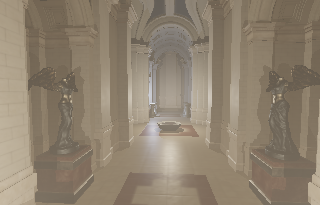
\includegraphics[width=.48\linewidth]{triangle-intersection/Sun-Temple.png}\hfill
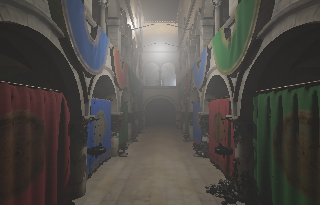
\includegraphics[width=.48\linewidth]{triangle-intersection/Sponza-Atrium.png}
\caption{正式编辑器第 24 帧的场景面板。左边的 Sun Temple 有 606\,376 个三角形和 8 个点光源；右边的 Sponza 有 262\,267 个三角形和 3 个点光源。两图都以 $320\times205$ 像素计算，雾沿视线分八步取样。}
\end{figure}

点光源从墙面朝灯检查遮挡，遇到一块挡光的砖就能返回。探针要找出沿途最近的表面，再读取那里的材质和光照。每帧更新 $12\times6\times7$ 个探针，每个探针朝六个方向取样，每方向两条射线，一共 6\,048 条。把探针照到的光分给屏幕上的像素时，只需读取附近探针，表中单列这一项作对照。

{\smalltable\noindent\begin{tabularx}{\linewidth}{@{}Xrrrr@{}}\toprule
GPU 时间（毫秒）& 逐灯照明 & 更新探针 & 读取探针 & 八步雾\\\midrule
Sun Temple，旧版     & 1.020 & 1.176 & 0.013 & 4.402\\
Sun Temple，共边检查 & 1.607 & 2.259 & 0.012 & 5.723\\
Sun Temple，共边检查与新分组 & 0.790 & 1.472 & 0.011 & 2.554\\\addlinespace
Sponza，旧版        & 0.911 & 1.189 & 0.012 & 3.666\\
Sponza，共边检查    & 1.511 & 2.139 & 0.012 & 4.633\\
Sponza，共边检查与新分组 & 0.795 & 1.035 & 0.012 & 2.571\\\bottomrule
\end{tabularx}\par}

第一次只改共边检查，神庙的探针更新耗时接近翻倍。最终版让一条射线经过的三角形共用一次投影准备，同时改了模型的分组方式。神庙的八步雾比旧版少用 1.848 毫秒，更新探针仍多用 0.296 毫秒；Sponza 的这两项均比旧版快。三版逐灯照明的线性 RGB 完全相同。按每通道 256 级导出最终版和旧版的面板图，神庙只有 8 个像素相差一级，Sponza 有 6 个，两图各有 65\,600 个像素。

使用 RTX 5070 Ti Laptop GPU、Debug x64 编辑器和 RenderDoc 1.47。每份捕获预热一次，再取 11 次 GPU 计时的中位数。表中四项各执行一次；神庙整帧有 70 次绘制、7 次计算，Sponza 有 125 次绘制、6 次计算。

\clearpage
\subsection{神庙模型的包围盒}
从高处看，神庙主体沿一条长廊展开。下图的每个灰点代表落在那一小块地面上方的三角形重心，越黑说明三角形越密。加载模型时，引擎给三角形分组，每组外面套一个能包住它们的长方体，沿分组一层层套下去，就得到一棵包围盒树。一条射线若连外面的盒子都碰不到，里面整组三角形就可以跳过。

\begin{figure}[H]\centering
\panelimage{.48\linewidth}{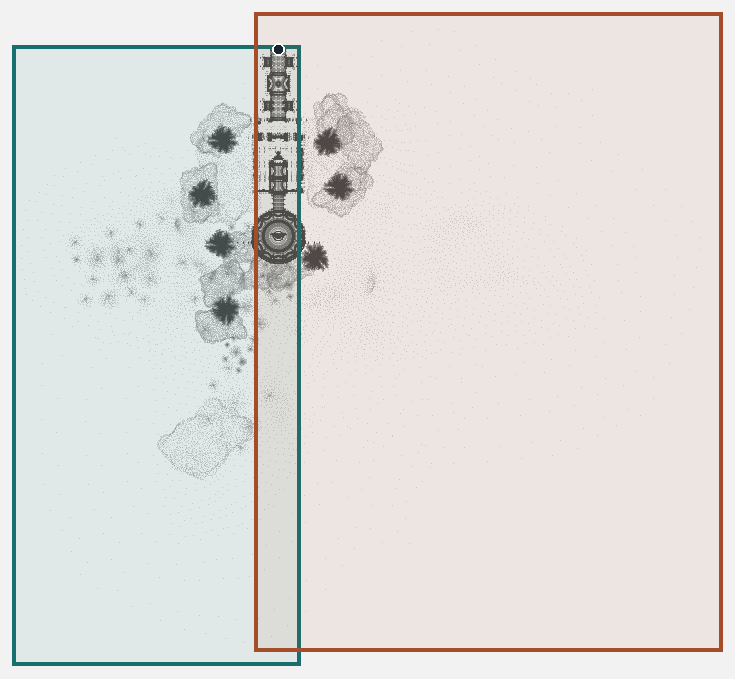
\includegraphics[width=\linewidth]{triangle-intersection/tree-median.png}\\[2pt]

\includegraphics[width=\linewidth]{triangle-intersection/tree-median-entry.png}}{按数量平分 · 每组 303\,188 个三角形}
\hfill
\panelimage{.48\linewidth}{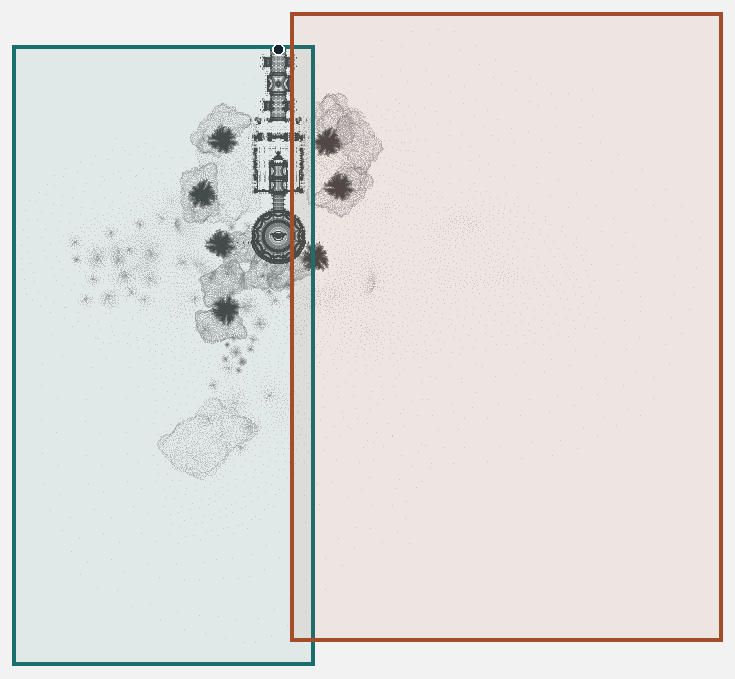
\includegraphics[width=\linewidth]{triangle-intersection/tree-area.png}\\[2pt]

\includegraphics[width=\linewidth]{triangle-intersection/tree-area-entry.png}}{按面积和数量分 · 538\,079 与 68\,297 个}
\caption{上排俯看整座神庙，下排放大长廊入口。青框和棕框是最外层包围盒分出的两组，取自 GPU 收到的节点。黑圆点是上一页的主相机。沿长廊向画面下方看，左图的两个盒子都覆盖了长廊中线，右图的棕框已退到旁边。}
\end{figure}

设一条射线沿长廊中线 $x=0$ 向前走，左右都不偏。左图两个盒子都跨过中线，即使只想查墙面到灯之间有没有遮挡，也可能要继续检查两组。右图把棕框的左边移到 $x=4.76$，这条射线可以跳过整个棕框。青框和棕框在水平方向重叠的宽度从 17.50 个场景单位缩到 9.09 个。图中只画了第一次分组，上一页的 GPU 计时包含整棵树。

从十二段中选一个分界时，引擎估算两边的检查量。把左盒表面积 $A_L$ 乘上它的三角形数 $N_L$，给右盒算同样的量，相加得到 $A_LN_L+A_RN_R$。同一个父盒内，选这个数最小的分界。较大的盒子更有机会被射线碰到，往它里面塞很多三角形，估算的工作就会增加。实现还会先存好每个三角形的包围盒和重心，排好顺序后再移动整份三角形数据。

在 Ryzen 9 8945HX 上交替运行两种建树方法，剔除一对预热后各取五次的中位数。神庙由 5.228 秒变为 3.066 秒，Sponza 由 2.281 秒变为 1.284 秒，耗时从已有三角形开始算到重排完成。每个节点占 48 字节。正式帧中神庙的节点数据从 12.00 降到 11.91\,MiB，Sponza 从 6.00 降到 5.12\,MiB。

\readings{\refitem{https://pbr-book.org/4ed/Primitives_and_Intersection_Acceleration/Bounding_Volume_Hierarchies}{PBRT 第四版 · 包围盒分割成本}\quad
\href{run:../profiling/triangle-intersection/README.md}{捕获、逐次 GPU 读数与 CPU 建树样本}}

\newpage
\fancyhead[R]{\sffamily\small\color{Muted}Vulkan / 镜面反射}
\section{镜头外的倒影}
镜子工作室的灯牌挂在相机后方。只查屏幕深度的 SSR 能看见墙和镜框，却找不到灯牌。打开「屏幕外反射」后，SSR 会先在屏幕上找。找不到时，显卡再沿反射方向查场景里的三角形，算出最近的表面朝镜子送来多少光。

\begin{figure}[H]\centering
\begin{minipage}{.45\linewidth}\centering\small\sffamily 只查屏幕\par\smallskip
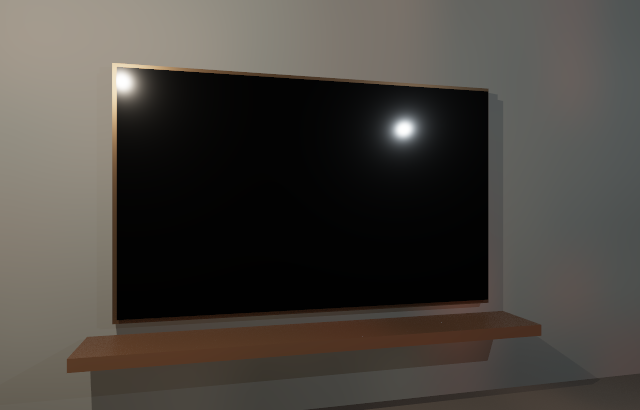
\includegraphics[width=\linewidth]{scene-reflections/mirror-screen.png}\par\vspace{3pt}
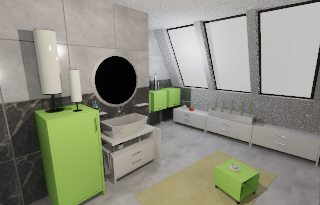
\includegraphics[width=\linewidth]{scene-reflections/bathroom-screen.png}
\end{minipage}\hfill
\begin{minipage}{.45\linewidth}\centering\small\sffamily 屏幕上找不到时再查场景\par\smallskip
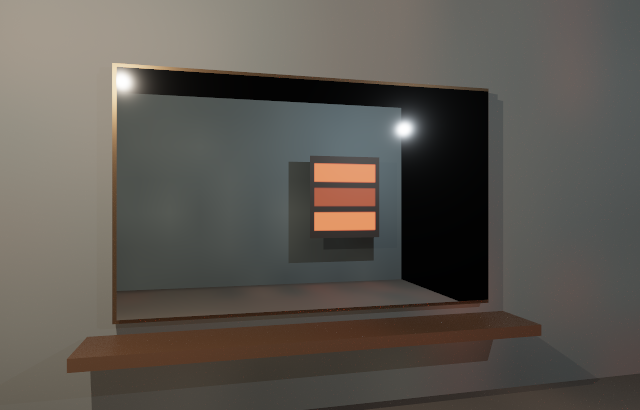
\includegraphics[width=\linewidth]{scene-reflections/mirror-scene.png}\par\vspace{3pt}
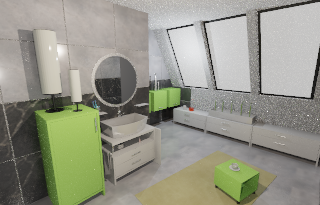
\includegraphics[width=\linewidth]{scene-reflections/bathroom-scene.png}
\end{minipage}
\caption{第 24 帧的场景面板，从 RenderDoc 回放导出。上排可以直接辨认镜中的横条灯牌。下排是 NVIDIA RTXGI 浴室，注意洗手盆上方的圆镜，右图里能看见对面墙上的明暗分界。}
\end{figure}

{\smalltable\noindent\begin{tabularx}{\linewidth}{@{}Xlrrr@{}}\toprule
场景和画幅 & 反射查找方式 & 事件编号 & 找到物体的像素 & GPU 毫秒\\\midrule
\mirrorTimingRows
\bottomrule\end{tabularx}\par}

两组都开启 SSR。找到物体的像素会在输出的第四个分量写入 1，照见黑框也算一次。用 RTX 5070 Ti Laptop GPU 运行 Debug x64 编辑器，在 RenderDoc 1.47 中预热一次，再回放 11 次。表中是单条反射计算命令的 GPU 耗时中位数。

浴室的画幅小，打开屏幕外反射后的用时却更长。除了统计像素，还值得数一数每条光线检查了多少三角形。下一步可以把屏幕上没找到物体的像素集中起来，再查场景。整理和追踪的时间都要计入，才能判断这样做能否更快。

{\small\color{Muted}逐次计时、原帧校验值和场景设置见 \path{output/profiling/scene-reflections/frames.json}。\par}

\newpage
\fancyhead[R]{\sffamily\small\color{Muted}Vulkan / 反射降噪}
\setlength{\parindent}{2\ccwd}
\ctexset{section={afterindent=true}}
\section{粗糙表面上的倒影}
浴室右侧的黑色窗框旁，灰墙上散布着亮点。墙面有一定粗糙度，每个像素的反射光线可能射向不同方向，一条碰到亮处，旁边一条却碰到暗处。开启「反射降噪」后，灰墙上的每个像素会借用附近墙面像素的倒影，墙面的底色仍取自原处。窗框和墙面的材质差异足够大，两边各自计算。

\begin{figure}[H]\centering
\begin{minipage}{.46\linewidth}\centering\small\sffamily 原始倒影\par\smallskip
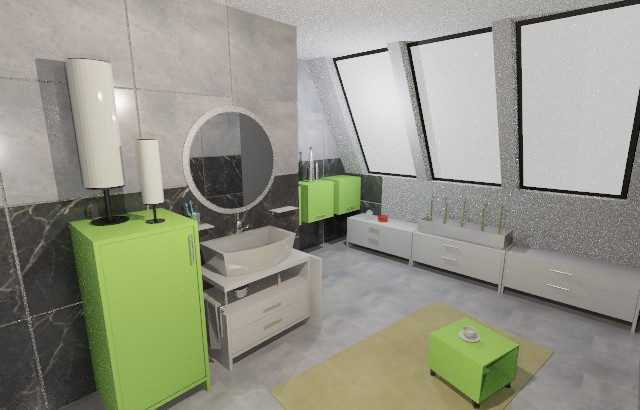
\includegraphics[width=\linewidth]{rough-reflections/small-off.png}
\end{minipage}\hfill
\begin{minipage}{.46\linewidth}\centering\small\sffamily 开启反射降噪\par\smallskip
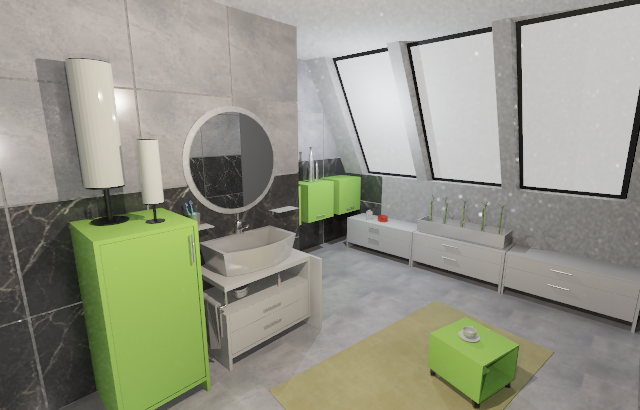
\includegraphics[width=\linewidth]{rough-reflections/small-on.png}
\end{minipage}\par\smallskip
\panelimage{.30\linewidth}{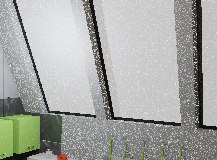
\includegraphics[width=\linewidth]{rough-reflections/detail-off.png}}{每像素一条光线}
\hfill\panelimage{.30\linewidth}{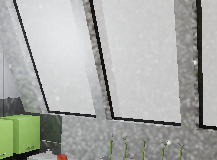
\includegraphics[width=\linewidth]{rough-reflections/detail-on.png}}{同一次采样，开启降噪}
\hfill\panelimage{.30\linewidth}{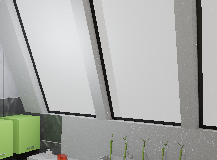
\includegraphics[width=\linewidth]{rough-reflections/detail-reference.png}}{每像素 256 次采样的平均值}
\caption{上排是 RTXGI Bathroom 在编辑器中的最终画面。下排单独查看 TAA 之前的窗框与墙面，三图使用相同的显示曲线。}
\end{figure}

固定相机与光照，对小画幅另取 256 组反射方向求平均，把它作为参照。把所有像素的线性红、绿、蓝三个分量分别和参照相减，平方后取平均，误差从 \roughRawMSE{} 降到 \roughFilteredMSE{}。将这 256 组分成两半，两张参照之间的同项误差为 \roughHalfMSE{}。

平均误差看不出哪条边变糊了。另一个测试让一面粗糙镜子照向亮灯牌，在镜子旁换上不同材质，每次都检查靠近分界处的两列像素。相邻材质换了颜色，或从金属换成非金属，这 192 个像素的结果都与旁边留空时相同。背景和理想镜面也分别比较了开关前后的颜色，每个像素都保持原值。浴室全图另查了每条反射光线是否命中物体，开启降噪后记录仍逐个相同。

\newpage
\section{反射追踪与降噪耗时}
两组渲染都使用浴室的原相机。第一组固定宽度为 640 像素，第二组按场景面板实际尺寸绘制。每种尺寸各抓两帧，只改「反射降噪」开关。RenderDoc 回放中，两帧追踪得到的原始反射逐字节相同，再比较它们各自花了多少时间。

{\smalltable\noindent\begin{tabularx}{\linewidth}{@{}Xlrrrr@{}}\toprule
画幅（像素）& 降噪 & 追踪（ms） & 降噪（ms） & 合计（ms） & 暂存（MiB）\\\midrule
\roughTimingRows
\bottomrule\end{tabularx}\par}

在 RTX 5070 Ti Laptop GPU 上捕获 Debug x64 编辑器，再用 RenderDoc 1.47 预热一次、回放 11 次。事件 556 负责追踪，开启时事件 568 执行降噪。「合计」先把同一次回放的耗时相加，再取中位数。两次捕获的追踪时间也有差异，所以最后两行的合计差值包含两部分。开关前后整帧都绘制 195 次，计算命令从 10 次增至 11 次。每个像素额外保存 16 字节的原始倒影，这块显存可以留给下一帧继续使用。

要判断打开浴室时该用哪个设置，我们还测了一整帧。关闭 RenderDoc 和 Vulkan 验证层，保留相同机位和面板原尺寸。三种设置轮换启动，各运行三次。每种设置记录 72 帧重新绘制的画面和 48 帧继续显示已有场景图的画面，从主线程开始处理这一帧一直计时到呈现返回，包含等待显卡的时间。

{\smalltable\noindent\begin{tabularx}{\linewidth}{@{}Xrrr@{}}\toprule
& \multicolumn{2}{c}{重新绘制（ms）}& 显示已有图（ms）\\
\cmidrule(lr){2-3}\cmidrule(l){4-4}
浴室的反射设置 & 中位数 & P95 & 中位数\\\midrule
\roughEditorRows
\bottomrule\end{tabularx}\par}

开启 SSR 的两行都允许射线离开屏幕后继续查询场景。重画时，这两行都比关闭 SSR 用时长。开启降噪的一组整帧中位数略低，但事件 568 本身占用了 0.350 毫秒。三轮启动测到的整帧用时也有起伏，暂不能用这组整帧差值判断降噪让引擎加速。

截帧还记录了 CPU 调用 \code{vkQueueSubmit} 把命令交给显卡用了多久。关闭降噪时，提交追踪用 \roughSubmitOff{} 微秒。开启时，提交追踪用 \roughSubmitOn{} 微秒，再提交降噪用 \roughSubmitFilter{} 微秒。这三个读数均来自捕获的第 24 帧，各只有一次。随后的等待以及显卡执行命令的时间需要另外计量。

浴室因此默认关闭 SSR。在场景面板打开 SSR 即可看到带降噪的屏幕内外倒影。后续可在 Vulkan 后端将追踪和降噪记进同一次提交，标清追踪写完、降噪才可读取的顺序。复测时沿用本页的两组计时，看减少一次提交和等待能省下多少整帧时间。

\readings{\href{run:../profiling/rough-reflections/bathroom.json}{GPU 逐次计时与误差}\quad
\href{run:../profiling/rough-reflections/editor-timing.json}{编辑器逐帧耗时}\quad
\href{run:../profiling/rough-reflections/editor-submits.json}{CPU 提交记录}\quad
\refitem{https://www.uni-ulm.de/fileadmin/website_uni_ulm/iui.inst.100/institut/Papers/atrousGIfilter.pdf}{Dammertz 等，HPG 2010，§2.2}}

\newpage
\fancyhead[R]{\sffamily\small\color{Muted}Vulkan / 镂空材质}
\section{Sponza 的镂空材质}

在 Sponza 长廊里，花盆中的叶片画在带纹理的三角形上。贴图里透明的部分应该让光穿过。旧版判断点光源有没有被挡住时，射线一碰到叶片的三角形就可能停下。修正后，射线先读命中位置的透明度，碰到孔洞就继续向前找。直接光、探针、反射和雾都用到了这项查询。

\begin{figure}[H]\centering
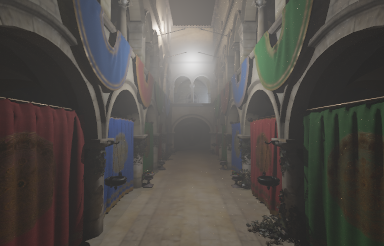
\includegraphics[width=.60\linewidth]{gi-mask/sponza-timing-view.png}
\caption{正式 Vulkan 编辑器实际计时的机位。RenderDoc 回放导出第 24 帧的面板颜色，画幅为 $384\times246$。两次捕获都开启分簇点光源、DDGI、GTAO、SSR、体积雾与 TAA。}
\end{figure}

用 RTX 5070 Ti Laptop GPU 运行 Debug x64 编辑器。保持模型、相机、灯光与渲染设置相同，在 RenderDoc 1.47 里将旧版和修正版各预热一次，再分别回放 11 次。下表记录每条计算命令在 GPU 上执行的毫秒数，取 11 次的中位数。末列为修正后减去修正前，正值表示这次测得的时间增加。

{\smalltable\noindent\begin{tabularx}{\linewidth}{@{}Xrrrr@{}}\toprule
计算命令 & 事件 & 整面遮挡 & 按贴图裁剪 & 差值（ms）\\\midrule
\maskTimingRows
\bottomrule\end{tabularx}\par}

两帧的场景和界面都合计绘制 228 次，计算命令均为 12 条。分簇点光源一行只测给表面算光的命令，前面把点光源分到各簇的时间另算。反射一行包括先查屏幕、再查场景的整个过程。表中雾的耗时最长，每条视线沿途取 8 处样本，还要检查各处能否收到灯光。

读取透明度会增加取样，光穿过小孔也会改变随后访问的三角形。这两项工作的次数目前没有分开统计。两份捕获中，点光源与雾耗时上升，探针与反射耗时下降。要分辨这些差值的来源，可以保持这套机位与设置，分别记录射线碰到几次镂空三角形、穿过了几个孔，再换几个机位核对。

\readings{\href{run:../profiling/gi-mask/sponza-timing.json}{原始帧位置、程序校验值及逐次耗时}\quad
\href{run:../../tests/replay_mask_timings.py}{回放脚本及复现命令}\\
\href{run:../profiling/gi-mask/sponza-reference.png}{同机位单帧与 256 次采样的反射参考图}\quad
\href{run:../profiling/gi-mask/sponza-reference.json}{参考图的取样记录与误差}}

\input{build/fine-mask-rows}
\newpage
\begingroup
\setlength{\parindent}{2em}
\ctexset{section/afterindent=true,subsection/afterindent=true}
\fancyhead[R]{\sffamily\small\color{Muted}Vulkan / 镂空边缘}
\section{贴图缩小后，哪些孔会消失}

Sponza 的一张镂空贴图有 $1024\times1024$ 个像素。每个像素除了颜色，还存有透明度。沿着光线找到叶片时，着色器在命中位置读取透明度。读数小于 0.5，光线就穿过叶片，继续检查后面的物体。

旧版把颜色和透明度一起缩到 $512\times512$。原图里相邻四个像素只留下一个，窄孔可能恰好落在另外三个位置。新版保留原尺寸的透明度，颜色仍用小图。两版使用相同的取样方法，位置落在四个像素之间时，离它近的像素占更大权重。

\begin{figure}[H]\centering
\begin{minipage}{.86\linewidth}\centering

\includegraphics[width=\linewidth]{fine-mask/mask-centers.png}\\[-1pt]
\makebox[.315\linewidth]{\small 原图}\hfill
\makebox[.315\linewidth]{\small 旧版取样}\hfill
\makebox[.315\linewidth]{\small 新版取样}
\end{minipage}
\caption{Sponza 材质 0 的同一块 $64\times64$ 区域。深绿表示挡光，浅色表示透光。中图的红色是旧版挡住的孔，橙色是旧版漏过的实体。三图在原图像素中心取样，放大时保持像素原形。为了看清差别，选取了这张图中错判最多的一块。}
\end{figure}

从实际截帧中读出材质数据，在 CPU 上逐一检查三张贴图的每个像素中心。表中的一次错判指同一个位置在源图与截帧里分别得到“挡光”和“透光”。原图坐标只计一次，同一片叶子出现在画面上多少次都不影响这里的计数。

{\smalltable\noindent\begin{tabularx}{\linewidth}{@{}Xrrrr@{}}\toprule
glTF 材质编号 & 使用它的三角形 & 旧版多挡的孔 & 旧版漏过的实体 & 新版错判数\\\midrule
0 & 31,436 & 10,692 & 10,893 & 0\\
3 & 3,472 & 3,931 & 4,061 & 0\\
20 & 32 & 1,750 & 2,142 & 0\\\bottomrule
\end{tabularx}\par}

在 3,145,728 个位置中，旧版共判错 33,469 处。新版从 GPU 读回来的三张透明度图逐字节与源图一致。画面中能看到多少差别，还取决于相机与光源的位置。将两个版本第 24 帧的面板图按每通道 256 级比较，94,464 个像素中有 616 个发生变化，最大相差 11 级。

\readings{\href{run:../profiling/fine-mask/mask-centers.json}{贴图文件、逐图结果和取样位置}\quad
\href{run:../../tests/sample_fine_masks.py}{取样与作图源码}\quad
\href{run:../profiling/fine-mask/sponza-frame.png}{同机位面板图与差值}\quad
\refitem{https://github.com/KhronosGroup/glTF-Sample-Assets/blob/e124e8d8d7330a5372bc2b4d00d39a4a9d7997ea/Models/Sponza/LICENSE.md}{Crytek Sponza 模型与许可}}

\newpage
\section{原尺寸透明度的存储与耗时}

三张图各保留 $1024\times1024$ 个透明度值，每个值用一个字节。每张图的开头再用八个字节保存宽和高。存放材质像素的 GPU 缓冲区从 50,331,712 字节增至 53,477,464 字节，差值恰好是 $3\times(1024^2+8)$。14 条材质记录共享这些贴图，仍合计 448 字节。两版的三角形与贴图坐标各占 16,785,088 字节，加速求交的树占 5,371,344 字节。这里统计 Vulkan 缓冲区长度，驱动分配的整块显存可能更大。

两版 Debug x64 编辑器使用同一机位，光照图均为 $384\times246$。用 RTX 5070 Ti Laptop GPU 捕获第 24 帧，保持分簇点光源、DDGI、GTAO、场景反射、8 步体积雾与 TAA 开启。RenderDoc 1.47 在旧、新、新、旧四轮中各预热一次，再测六次，每个版本留下 12 个样本。两帧均有 228 次绘制和 12 次计算调度。

{\smalltable\noindent\begin{tabularx}{\linewidth}{@{}Xrrrrr@{}}\toprule
GPU 命令 & 事件 &\multicolumn{2}{c}{旧版（ms）}&\multicolumn{2}{c}{新版（ms）}\\
\cmidrule(lr){3-4}\cmidrule(l){5-6}
& & 中位数 & P10--P90 & 中位数 & P10--P90\\\midrule
\fineGpuRows
\bottomrule\end{tabularx}\par}

P10--P90 表示中间八成样本的用时范围。复制表面位置和法线的命令没有取样透明度，耗时仍有波动。两版的反射和雾都测到了彼此重叠的用时范围。

{\smalltable\noindent\begin{tabularx}{\linewidth}{@{}Xrr@{}}\toprule
编辑器计时 & 旧版 & 新版\\\midrule
\fineCpuRows
\bottomrule\end{tabularx}\par}

关闭 RenderDoc 和 Vulkan 验证层，交替启动两个版本共六次。每版有 72 帧重画场景，另有 48 帧沿用已有面板图。重画一帧的中位用时增加了 1.19 ms，其中包含等待显卡与显示窗口的时间。进程 CPU 时间由 Windows 累加所有线程从启动到退出的用时，包含导入模型和运行 56 帧。队列提交耗时取自两份截帧，各只有一帧。

\readings{\href{run:../profiling/fine-mask/gpu.json}{GPU 事件、缓冲区长度和逐次用时}\quad
\href{run:../profiling/fine-mask/editor.json}{独立进程与逐帧记录}\quad
\href{run:../profiling/fine-mask/final-frame.json}{最终版同机位复核}\\
计时版本为 \code{532eca6d7921} 和 \code{7c1c4c8e2382}。最终版 \code{435a0ada6466} 单独核对材质与输出图。}
\clearpage
\endgroup

\input{build/ssaa-rows}
\section{SSAA 的四个着色样点}

Sponza 中庭的场景面板输出 $384\times246$ 个像素。打开「SSAA 2×2」后，模型表面、光照和屏幕效果先画成 $768\times492$；同一块面板像素对应四个内部位置。图中两次运行均取编辑器第 24 帧。镜头、灯光和曝光设置相同，右侧树叶与石地的局部按同一倍率放大。

\begin{figure}[H]\centering
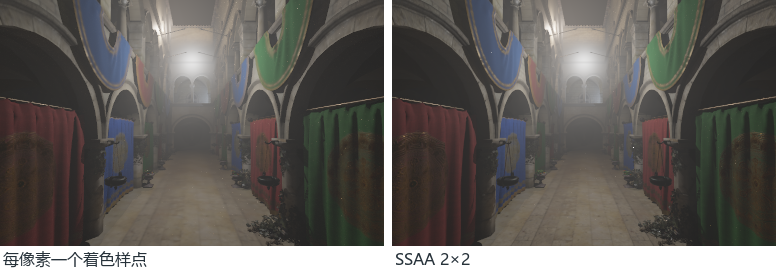
\includegraphics[width=.96\linewidth]{ssaa/sponza.png}\par\vspace{5pt}
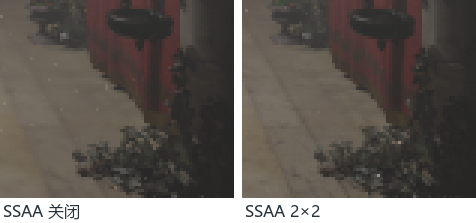
\includegraphics[width=.64\linewidth]{ssaa/foliage.png}
\caption{上图来自 Vulkan 编辑器最终送往场景面板的颜色图。下图取原图从 $(222,173)$ 开始的 $78\times66$ 像素，放大三倍。房间内的 TAA、DDGI、GTAO、反射和雾均参与这次绘制。}
\end{figure}

\ssaaExample\par

\ssaaVerified\par

同一机位另用前一版程序画了一次。无论关闭还是开启 SSAA，两版输出的 8 位颜色图均逐像素相同。要观察新算法怎样保留远处的细线，可以看相机移过斜纹时的连续帧。\par

\readings{\href{run:../profiling/ssaa/on-replay.json}{四个样点与逐像素核验}\quad
\href{run:../profiling/ssaa/off-replay.json}{关闭时的回放}\quad
\href{run:../profiling/ssaa/sponza.png}{完整画面}\quad
\href{run:../validation/mask-footprint-compare-rank/diagonal-motion.png}{移动相机经过斜纹}}

\newpage
\section{Sponza 的显存与耗时}

这次使用 Debug x64 编辑器（\texttt{\ssaaBuild}）和 RTX 5070 Ti Laptop GPU。实际编辑视口为 $1391\times892$，场景面板的输出宽度固定为 384。103 次绘制写入供光照读取的模型表面，另有 103 次供编辑器拾取、22 次画界面。开关 SSAA 的绘制次数相同，打开后，光照和屏幕效果需要处理四倍的内部像素。

{\smalltable\noindent\begin{tabularx}{\linewidth}{@{}Xrr@{}}\toprule
渲染资源 & 关闭 & SSAA 2×2\\\midrule
\ssaaStorage
\bottomrule\end{tabularx}\par}

缓冲区取 RenderDoc 在捕获中列出的长度，图像取纹理条目的字节数。两帧都登记了 232 个缓冲区和 319 张图像，合计多出约 75 MiB，其中约 65 MiB 来自缓冲区。这个差值反映两份截帧列出的资源大小；要测驱动实际驻留的显存峰值，还需跟踪分配与释放。

{\smalltable\noindent\begin{tabularx}{\linewidth}{@{}Xrr@{}}\toprule
测量范围（毫秒） & 关闭 & SSAA 2×2\\\midrule
\ssaaTimes
\bottomrule\end{tabularx}\par}

GPU 时间来自 RenderDoc 1.47 的事件计数器。按关、开、开、关回放，每轮先预热一次，再取六次；将同组事件在一次回放内相加，再取该设置 12 次结果的中位数。绘制与计算的合计覆盖列出的事件，帧中另有清屏、复制、等待与呈现。提交队列的数字是截帧当次主机调用 \code{vkQueueSubmit} 的用时之和，各一帧。

整帧数据来自未挂 RenderDoc 和 Vulkan 验证层的六次独立启动。每种设置先后启动三次。面板最后一次调整大小后，每次跳过前八帧，记录 24 帧重画，另记录 16 帧沿用已有面板图。整帧计时包括主线程等待 GPU 和窗口呈现。P95 表示约 95\% 的样本用时低于该值。两种设置的计算派发相差约 17 毫秒。若要缩短本场景的重画时间，可先分别测量反射与雾在两种分辨率下的用时。\par

\readings{\href{run:../profiling/ssaa/gpu.json}{GPU 每次回放与提交时间}\quad
\href{run:../profiling/ssaa/editor.json}{编辑器逐帧耗时}\quad
\href{run:../profiling/ssaa/on-capture.json}{程序、设置与原始帧校验值}\quad
\href{run:../../tests/profile_ssaa.py}{复现脚本}}

\end{document}
